% !TeX spellcheck = lt
\documentclass{VUMIFInfMagistrinis}
\usepackage{algorithmicx}
\usepackage{algorithm}
\usepackage{algpseudocode}
\usepackage{amsfonts}
\usepackage{amsmath}
\usepackage{bm}
\usepackage{color}
\usepackage{listings}
\usepackage{etoolbox}
\usepackage{graphicx}
\usepackage{hyperref}
\usepackage{setspace}

\newcommand{\argmax}{\operatornamewithlimits{argmax}}
% Titulinio aprašas
\university{Vilniaus universitetas}
\faculty{Matematikos ir informatikos fakultetas}
\department{Informatikos katedra}
\papertype{Magistro baigiamasis darbas}
\title{Šalto starto problemos rekomendacinėse sistemose sprendimas naudojant socialinių tinklų duomenis}
\titleineng{Applying Social Network Data for Cold Start Problem in Recommender Systems}
\status{II kurso Informatikos studentas}
\author{Andrius Juškevičius}
\supervisor{lekt. Rimantas Kybartas}
\reviewer{prof. habil. dr. Antanas Žilinkskas}
\date{Vilnius – \the\year}

% Nustatymai
% \setmainfont{Palemonas}   % Pakeisti teksto šriftą į Palemonas (turi būti įdiegtas sistemoje)
\bibliography{bibliografija}

\begin{document}

\maketitle

%% Padėkų skyrius
% \sectionnonumnocontent{}
% \vspace{7cm}
% \begin{center}
%     Padėkos asmenims ir/ar organizacijoms
% \end{center}

\sectionnonumnocontent{Santrauka}
Žmonės priimdami sprendimus dažnai pasikliauja draugų ir pažįstamų rekomendacijomis. Vienas iš rekomendacinių sistemų (toliau - RS) metodų - bendradarbiavimo filtravimas (angl. collaborative filtering, toliau BF) nors ir imituoja žmonių tarpusavio panašumą, negali identifikuoti, ką žmogus pažįsta, o ko ne. Socialinių tinklų duomenys užpildo šią spragą ir leidžia RS pateikti rekomendacijas atsižvelgiant ir į žmonių tarpusavio santykį. 
\newline
\indent
Šiame darbe pateikta glausta rekomendacinių sistemų apžvalga, išnagrinėtas bendradarbiavimo filtravimo algoritmas, pristatyta šalto starto problema bei apžvelgtos socialinio tinklo duomenų taikymo galimybes sprendžiant šią problemą. Taip pat pasiūlyti trys nauji, socialinių tinklų duomenų panaudojimu besiremiantys metodai, kuriuos taikant galima spręsti šalto starto problemą.
% Nurodomi iki 5 svarbiausių temos raktinių žodžių (terminų).
% Vienas terminas gali susidėti iš kelių žodžių.
\raktiniaizodziai{rekomendacinė sistema, bendradarbiavimo filtravimas, socialinis tinklas, šaltas startas, pasitikėjimas}   

\tableofcontents

\sectionnonum{Įvadas}
\linespread{1.5}
\selectfont
\indent
Kaskart, kai kažko ieškome, tiksliai patys nežinodami, ko - susiduriame su rekomendacijos poreikiu. Iš esmės, didžioji dalis dalykų apie kuriuos žinome, mums kažkada buvo viena ar kita forma pasiūlyta ar nurodyta. Taigi, didelė dalis pasaulio pažinimo proceso įvyksta rekomendacijų dėka. Rekomendacija, kaip reiškinys, gali įgyti įvairias, dažniausiai socialines, formas - informacijos galime gauti iš artimųjų arba tam tikrų atstovų (pavyzdžiui, finansų patarėjo arba konsultanto). Kita forma, apie kurią ir yra šis darbas, yra skaitmeninė - rekomendacinių sistemų (toliau - RS) generuojamos rekomendacijos skaitmeninėje erdvėje siekia palengvinti naudotojo patirtį renkantis jį dominančius elementus iš prieinamos aibės. Šios rekomendacijos gali ne tik palengvinti paieškos procesą, bet ir pasiūlyti bei sudominti naudotoją tokiais elementais, apie kuriuos naudotojas nė nenutuokė. Šis bruožas yra ypač aktualus kitai šio santykio pusei - siūlytojui (pavyzdžiui, pardavėjui) dėl akivaizdžių priežasčių - jis tampa labiau matomas, žinomesnis, galų gale jis gali gauti materialinės naudos.
\newline
\indent
RS plačiai taikomos muzikos, kino ir elektroninės prekybos platformose. Vietoj įprastos paieškos šios sistemos siūlo elementus pasiremdamos naudotojų elgesio istorija. Vienas labiausiai naudojamų metodų - bendradarbiavimo filtravimas (angl. Collaborative Filtering, toliau - BF). Aibė sėkmingų interneto įmonių (pavyzdžiui, Amazon.com, Netflix.com, Last.fm) pritaikė BF metodus tam, kad padidinti naudotojų pasitenkinimą jų siūlomu produktu. Taikant BF daroma prielaida, kad istoriškai panašūs naudotojai išliks tokie ir ateityje. Taigi, esminė problema, kurią reikia spręsti - naudotojų panašumo vertinimas. Filtravimo procesas remiasi jau turimais duomenimis, kurie dėl problemos prigimties yra labai reti - sistemoje gali būti tūkstančiai naudotojų ir dar daugiau elementų, tačiau kiekvienas naudotojas dažniausiai būna įvertinęs tik labai mažą visų elementų dalį, taigi panašumo įvertinimas tampa iššūkiu. Negana to, kai sistemoje atsiranda naujas naudotojas, pradžioje apie jį žinoma per mažai, kad būtų galima pateikti patikimas rekomendacijas. Ši problema dar kitaip vadinama šalto starto (angl. cold start problem). Ji yra ypač svarbi ir dėl to, kad, jeigu naujas naudotojas per pakankamai trumpą laiką neįsitikins sistemos nauda, labai tikėtina, kad jis niekada ja nebesinaudos.
\newline
\indent
Ieškant šios problemos sprendimo būdų buvo atlikta nemažai tyrimų apie hibridines RS. Šių hibridinių RS esmė - taikant BF panaudoti informaciją apie elementų turinį. Turiniu pagrįstas RS nagrinėja atskira šaka, apie kurią šiame darbe nebus kalbama. Nors hibridinės RS ir išsprendžia dalį problemos, tačiau turi vieną esminį trūkumą - hibridinė RS yra labai priklausoma nuo konteksto, kuriame ji naudojama, kitaip sakant, ji yra neuniversali. Be to, kai kurioms dalykinėms sritims yra labai sudėtinga apibūdinti naudotojo susidomėjimo elemento atributus, taigi neįmanoma sukurti tokios RS.
\newline
\indent
Šio darbo tikslas – pasiūlyti metodą, kuriuo remiantis būtų galima išspręsti duomenų nepakankamumo problemą juos papildant duomenimis iš socialinių tinklų. Šie duomenys puikiai panaudojami pasitikėjimu pagrįstose RS. Pasitikėjimas gali būti traktuojamas kaip alternatyvus dydis panašumui. Šie du dydžiai skiriasi:
\begin{itemize}
	\item pasitikėjimas nebūtinai yra išskaičiuojamas iš duomenų - jis gali būti išreikštas tiesiogiai.
	\item pasitikėjimas turi kryptį - tai yra naudotojas $u_1$ gali pasitikėti $u_2$ ne tiek pat, kiek $u_2$ $u_1$.
\end{itemize}
Pasitikėjimo tinklas - grafas, kurio viršūnės vaizduoja naudotojus, briaunos - santykius tarp jų, o briaunų svoriai - pasitikėjimo įverčius. Toks tinklas ir bus pamatas siūlomiems metodams, kaip spręsti šalto starto problemą, kai nepakanka duomenų naudotojų panašumui nustatyti.
\newline
\indent 
Literatūros apžvalgoje suformuluoti bendradarbiavimo filtravimo naudotoju pagrįstu ir daiktu pagrįstu metodų apibrėžimai, pristatyta šalto starto problema ir aprašyti įvairių autorių pasiūlyti metodai šiai problemai spręsti. Tyrimai apie socialinių tinklų duomenų panaudojimą bus aptarti plačiau ir pristatyti jau atlikti darbai šia problemos sprendimo kryptimi. Taip pat gilinamasi į socialinių tinklų duomenų panaudojimo galimybes siekiant panaikinti (arba sušvelninti) šalto starto problemos efektą. Kitame skyriuje pristatytas būdas, kaip galima generuoti socialinių tinklų duomenis ir pasiūlyti trys nauji metodai naudojami RS su socialinių tinklų duomenimis - bendrų kaimynų metodas, atsižvelgiantis tik į ryšių egzistavimą tarp naudotojų, sričių panašumo metodas, kuris taikomas RS su kategorijomis, ir pasitikėjimo interpoliavimo metodas, kurio esmė - prognozuoti naudojo tarpusavio pasitikėjimą remiantis "paslėptais" RS duomenimis (juos naudojame generuodami RS duomenis). Trečiame skyriuje pateikta pasiektų rezultatų santrauka ir išvados.
%Toliau bus atlikta detali rezultatų analizė ir siūlyto metodo palyginimas su kitų tyrėjų anksčiau pasiūlytais RS metodais, aptarti pristatytų metodų privalumai ir trūkumai.


\section{Litratūros apžvalga}
\subsection{Bendradarbiavimo filtravimas}
%Vertinimas išplaukia iš konteksto
\subsubsection{Bendradarbiavimo filtravimo metodas}
Visų pirma, suformuluokime RS sprendžiamą problemą formaliai taip, kaip tai padaryta \cite{2}. Vartotojų aibė pažymėkime $U$ ir elementų aibę $I$. Be to, pažymėkime $R$ aibę sistemoje turimų reitingų ir $S$ – aibę galimų reikšmių, kurias gali įgyti reitingas (pvz. $S=[1,5]$). Taip pat, tarkime, kad vienas reitingas $r_{ui}$ gali būti priskirtas vienam elementui $i \in I$ vieno naudotojo $u \in U$. Vartotojų poaibį, kuris yra įvertinęs elementą $i$, pažymėkime $U_i$. Analogiškai, $I_u$ pažymėkime aibę elementų, kuriuos yra įvertinęs naudotojas $u$. Daiktų, kuriuos yra įvertinę abu naudotojai $u$ ir $v$, aibę $I_u \and I_v$ pažymėkime $I_{uv}$. Analogiškai, $U_{ij}$ žymi aibę naudotojų, kurie yra įvertinę tiek elementą $i$, tiek $j$. Dvi dažniausiai sutinkamos problemos – geriausios ir geriausių $N$ rekomendacijos problema. Vienas būdų spręsti šias problemas yra įvertinti funkciją $f: U \times I -> S$, kuri nuspėja reitingą $f(u,i)$. Ši funkcija tada yra naudojama naudotojo $u_a$ rekomendacijai elemento $i^*$, kuriam įvertinamas reitingas turi didžiausią reikšmę $i^*= \arg \max \limits_{j \in \frac{I}{I_u}} f(u_a,j)$. 
RS galima modeliuoti dviem būdais:
\begin{itemize}
	\item Turiniu-pagrįstų metodų esmė – identifikuoti charakteristikas, kuriomis pasižymėjo elementai, kuriuos naudotojas įvertino palankiai praeityje ir tada naudotojui rekomenduoti kitus elementus su panašiomis charakteristikomis.
	\item Bendradarbiavimo-filtravimu pagrįsti metodai rekomenduoja elementus, kurie patiko naudotojams, turintiems panašias pirmenybes. BF metodai remiasi tik naudotojų suteiktais reitingais. Jie ieško panašumų tarp naudotojų pirmenybių ir tai lemia dvi geras savybes, kuriomis nepasižymi turiniu pagrįsti metodai
	\begin{itemize}
		\item įžvalgumas - siūlomi ne tik akivaizdūs pasiūlymai, bet ir netikėti (t.y. tokie, kokių naudotojas kitomis aplinkybėmis turbūt nerastų)
		\item pritaikymas skirtingose srityse, elementu pagrįstos rekomendacijos reikalauja specifinių srities parametrų duomenų (pvz., kiek tam tikras filmas yra komedija, kiek drama)
	\end{itemize}
	Bendradarbiavimo filtravimo sąvoką pirmąsyk panaudojo Goldberg \cite{16}. Šis metodas remiasi  artimiausių kaimynų metodu ir naudoja duomenis tiesiogiai generuojant rekomendacijas. Toliau darbe bus nagrinėjami būtent šiai klasei priklausantys metodai.
\end{itemize}
Bendradarbiavimo filtravimu pagrįsta reitingo prognozės esmė ta, kad parenkami artimiausi naudotojo kaimynai. Vartotojų tarpusavio artumas nustatomas naudojant panašumo metrikas, kurios bus aprašytos vėliau skyriuje \ref{ssec:sim}. Šią prognozę galima atlikti dvejopai:
\begin{itemize}
	\item Taikant artimiausių kaimynų regresiją, reitingas įvertinamas skaičiuojant pasvertą artimiausių kaimynų vidurkį.
	\item Taikant artimiausių kaimynų klasifikaciją, elemento reitingas parenkamas toks pats, kokį jam yra suteikęs artimiausias naudotojo kaimynas
\end{itemize}

\indent
Pagrindinis turiniu pagrįsto prieš naudotoju pagrįstą reitingo prognozavimo trūkumas yra tas, kad tokiu būdų sugeneruotos rekomendacijos yra nors ir tikslios, tačiau nelabai vertingos, nes rekomenduojami elementai pernelyg panašūs į tuos, kuriuos naudotojas jau žino. Šią problemą galima vertinti kaip pernelyg didelio pritaikymo (angl. over-specialization) problemą arba kaip įžvalgumo (angl. serendipity) stygių. Be to, naudotoju pagrįstas metodas yra paremtas realiu žinių perdavimo iš lūpų į lūpas modeliu, todėl, tikėtina, geriau modeliuoja žinių išgavimą.
\newline
\indent
Norėdami prognozuoti naudotojo $u$ reitingą elementui $i$, imame $k$ artimiausių kaimynų $N_i(u, k)$ ir ieškome jų vidurkio.
\begin{equation}
\hat{r}_{ui} = \frac{1}{N_i(u, k)}\sum \limits_{v \in N_i(u, k)} r_{vi}
\end{equation}
Ši formulė neatsižvelgia į naudotojų panašumą. Būtų neteisinga vertinti visus kaimynus vienodai, kai kai kurie yra panašūs į naudotoją $u$, o kai kurie visiškai nepanašūs. Čia įtraukiame svorių sąvoką. Svoriai gali reikšti arba panašumą (plačiau -\ref{ssec:sim}), arba, kaip vėliau bus parodyta, vieno naudotojo pasitikėjimą kitu, apie kurį rašoma \ref{ssec:trust}.
\begin{equation}\label{eq:1}
\hat{r}_{ui} = \frac{\sum \limits_{v \in N_i(u, k)} w_{uv} r_{vi}}{\sum \limits_{v \in N_i(u, k)} |w_{uv}|}
\end{equation}
Šioje formulėje naudojamas svertinis vidurkis yra dažniausiai praktikoje taikomas, paprastas ir tikslus būdas nustatyti prognozei, tačiau lieka klausimas - į kiek kaimynų reikia atsižvelgti. GroupLens sistemoje visi $U \setminus \{u\}$ laikomi kaimynais; kitose sistemose kaimynai parenkami pagal panašumo slenkstį. Tinkamas kaimynų skaičiaus parinkimas leidžia įvertinti tikslesnes prognozes, nes taip sumažinamas kaimynų su maža koreliacija keliamas triukšmas. Dar kitas būdas - atsižvelgiant į dalykinę sritį parinkti konstantą. Geriausią kaimynų parinkimo strategiją galima išsiaiškinti tiesiog paeksperimentavus su konkrečiais duomenimis, nes įprastai RS viena nuo kitos labai skiriasi tiek dėl dalykinės srities subtilybių, tiek dėl RS dalyvaujančių naudotojų.  

\subsubsection{Šalto starto problema}
Šalto starto problema susijusiu su nepakankamu duomenų kiekiu. Šią problemą galima išskirti į dvi dalis:
\begin{itemize}
	\item naudotojo šaltas startas
	\item elemento šaltas startas
\end{itemize}
\indent 
Toliau bus rašoma tik apie naujo naudotojo problemą. Bendradarbiavimo filtravimu pagrįstuose metoduose, norint pateikti prasmingą rekomendaciją, visų pirma reikia suformuoti aiškų naudotojo pirmenybių vaizdą. Naujam naudotojui to padaryti faktiškai neįmanoma. Šia problemą galima spręsti visai negeneruojant rekomendacijų arba teikti rekomendacijas remiantis naudotojo profiliu - gyvenamąja vieta, amžiumi, lytimi ir panašiai. Dar kitas būdas - įvertinti trūkstamus duomenis - ir yra šio darbo esminis tyrimo objektas.
\subsubsection{Naudotojų panašumo apskaičiavimas}\label{ssec:sim}
Jau anksčiau buvo minėta, kad norint rasti prognozuojamą naudotojo $u$ tam tikram elementui $i$ suteikiamą reitingą, reikia žinoti svorius, kuriais matuojama kitų panašių naudotojų įtaka galutinei prognozei. Vienas šių svorių įvertinimo būdų - naudotojų panašumo išskaičiavimas iš reitingų matricos. Toliau pristatomi metodai, kurie padeda įvertinti naudotojų panašumą. Pyrsono, Spearmano koreliacija ir kosinuso panašumas detaliau aprašyti \cite{2}.
\subsubsubsection{Pyrsono koreliacija}
Pyrsono koreliacija skirta statistinės koreliacijos radimui:
\begin{equation}
s(u,v) = \frac{\sum \limits_{i\in I_u \cap I_v }(r_{u,i}-\bar{r}_u)(r_{v,i}-\bar{r}_v)}{\sqrt{\sum\limits_{i \in I_u \cap I_v }(r_{u,i} - \bar{r}_u)^2}\sqrt{\sum\limits_{i \in I_u \cap I_v }(r_{v,i} - \bar{r}_v)^2}}
\end{equation}
Šis metodas susiduria su sunkumais, kai reikia paskaičiuoti panašumą tarp naudotojų, kurie bendrai yra įvertinę mažai elementų. Galima išeitis - nustatyti slenkstį, nuo kurio koreliacija būtų mažinama. Taigi panašumą $s(u,v)$ tokiu atveju reiktų dauginti iš baudos funkcijos 
\begin{equation}
min\{|I_u \cap I_v|, 1\}
\end{equation}
\subsubsubsection{Apribota Pyrsono koreliacija}
Kai kalbame apie šį metodą, pereiname nuo tolydinio prie kategorinio parametrų vertinimo. Be to, atsižvelgiama į nuokrypį ne nuo vidurkio, o nuo abejingumo įverčio. Jeigu turime reitingų skalę nuo 1 iki 7, tada 4 reiškia abejingumą. Pažymėkime $r_x = 4$. Tada Shardanand ir Maes pasiūlyta apribota Pyrsono koreliacija randama taip
\begin{equation}
s(u,v) = \frac{\sum \limits_{i\in I_u \cap I_v }(r_{u,i}-r_z)(r_{v,i}-r_z)}{\sqrt{\sum\limits_{i \in I_u \cap I_v }(r_{u,i} - r_z)^2}\sqrt{\sum\limits_{i \in I_u \cap I_v }(r_{v,i} - r_z)^2}}
\end{equation}
\subsubsubsection{Spearmano rango koreliacija}
Spearmano rango koreliacija panaši į Pyrsono koreliaciją, vienintelis skirtumas toks, kad skaičiuojant Spearmano koreliaciją, naudotojo reitingai yra surūšiuojami didėjimo tvarka, jiems priskiriami rangai - mažiausią reikšmę turintis reitingas gauna reikšmę 1. Tokiu būdu išvengiama reitingų normalizavimo problemos. Šis metodas veikia ne itin gerai, kai yra mažas galimų reikšmių skaičius, be to skaičiavimo požiūriu reikalaujantis daugiau resursų dėl surūšiavimo žingsnio.
\subsubsubsection{Kosinuso panašumas}
Šis metodas skiriasi nuo ankstesnių tuo, kad yra į problemą žiūrima ne iš statistinio, o iš tiesinės algebros požiūrio taško. Vartotojai atvaizduojami kaip $|I|$ dimensijų turintys vektoriai, o panašumas apskaičiuojamas, kaip kosinuso atstumas tarp dviejų reitingo vektorių. Jis randamas sudauginant šiuos vektorius ir padalinant iš $L2$ (Euklido) normų sandaugos:
\begin{equation}
s(u,v) = \frac{\boldsymbol{r}_u \cdot \boldsymbol{r}_v}{||\boldsymbol{r}_u||_2 ||\boldsymbol{r}_v||_2}
\end{equation}
\subsubsubsection{Euristinis PIP panašumo matas}
Euristinis panašumo matas pasiūlytas \cite{7} kreipia dėmesį į šalto starto problemą. Dažniausias šalto starto problemos sprendimo būdas - naudoti hibridines RS, kurios naujiems naudotojams rekomendacijas pateikia naudodamos turinio informaciją ir tik surinkus pakankamai duomenų apie naudotoją, įjungiamas BF režimas. Ši panašumo metrika atsižvelgia į šalto starto problemą panašumą apskaičiuodama remdamasi trimis faktoriais - panašumu, poveikiu, populiarumu.
\begin{equation}
s(u_i, u_j)= \sum \limits_{k \in C, j}\boldmath{PIP}(r_{i,k}, r_{j,k})
\end{equation}
čia $r_{ik}$ ir $r_{jk}$ reitingai elementui $k$ nuo naudotojų $i$ ir $j$ atitinkamai, $PIP(r_{ik}, r_{jk})$ - $PIP$ reikšmė reitingams $r_{ik}$ ir $r_{jk}$
\begin{equation}
PIP(r_1,r_2) = Proximity(r_1,r_2) \times Impact(r_1,r_2) \times Popularity(r_1,r_2)
\end{equation}
Detalesnis aprašymas, kaip randamos šios reikšmės yra \cite{7}.
\subsubsubsection{Panašumas su svoriais}
\cite{13} Said pastebėjo, kad dažniausiai naudojami panašumo matai (Pyrsono koreliacija, kosinuso panašumas) turi tokį trūkumą, kad jie neatsižvelgia į bendrai įvertintų elementų populiarumą - bendrai įvertinti populiarūs (įvertinti daugelio naudotojų) elementai vertinamam panašumui turėtų daryti mažesnę įtaką negu retai vertinami. Šį trūkumą siūloma spręsti panašumo matuose įvedant populiarumo svorius.
\newline
\indent
Tokiu būdu randama Pyrsono koreliacija atrodytų taip:
\begin{equation}
s_w(u,v) = \frac{\sum \limits_{i\in I_u \cap I_v }w_i^s(r_{u,i}-\bar{r}_u)(r_{v,i}-\bar{r}_v)}{\sqrt{\sum\limits_{i \in I_u \cap I_v }w_i^s(r_{u,i} - \bar{r}_u)^2}\sqrt{\sum\limits_{i \in I_u \cap I_v }w_i^s(r_{v,i} - \bar{r}_v)^2}}
\end{equation}
ir kosinuso panašumas:
\begin{equation}
s_w(u,v) = \frac{\sum \limits_{i\in I_u \cap I_v} w_i^s \cdot r_{u,i} \cdot r_{v,i}}{\sqrt{\sum\limits_{i \in I_u} w_i \cdot r_{u,i}^2}\sqrt{\sum\limits_{i \in I_v} w_i^s \cdot r_{v,i}^2}}
\end{equation}
o svoriai $w_i^s$ gali randami būti randami tokiais būdais:
\begin{equation}
w_i^{s,inf} = \log \frac{|U|}{|U_i|}
\end{equation}
\begin{equation}
w_i^{s,lin} = 1 - \frac{|U_i|}{|R|}
\end{equation}
Čia $|U|$ - naudotojų skaičius, $|U_i|$ - naudotojų, įvertinusių elementą $i$ skaičius, $|R|$ reitingų skaičius.
\newline
\indent
Šaltinyje \cite{13} parodyta, kad šis metodas geriausiai veikia vartotojams "po šalto starto" (angl. post cold start users), kai reitingų skaičius yra tarp 20 ir 80, kitiems rėžiams rezultatai buvo labai panašūs į tuos, kurie buvo gauti naudojant Pyrsono koreliaciją be svorių.  

\subsection{Socialiniai tinklai ir pasitikėjimu pagrįstos rekomendacinės sistemos}
\subsubsection{Socialiniai tinklai ir pasitikėjimo sąvoka}
% reikia gražiai įpinti šitą gabalą čia.
Socialinis tinklas - virtuali bendruomenė, kurios nariai bendrauja ir dalinasi tarpusavyje informacija. Žmonės tokiose bendruomenėse būna susiję - arba abipusiu (draugų), arba vienpusiu (pasekėjų) ryšių.
%Šiame tyrime, mus domina abipusis ryšys.
Pasitikėjimu pagrįstų RS tikslas - įvertinti, kiek pasitikėjimo turi vienas naudotojas kitu, kai turimas pasitikėjimo tinklas (angl. web of trust). Įprastai toks įvertis randamas taikant propagavimo ir agregavimo operatorius. Propagavimo operatoriai nulemia, kaip bus elgiamasi su tranzityvumu. Kol kas nesigiliname į tai, kaip gaunami pasitikėjimo įverčiai, laikome juos duotais. 
\indent
\begin{itemize}
	\item Vienas dažniausiai naudojamų propagavimo operatorių (ypač, kai kalbame apie tikimybinį požiūrį) yra daugyba. Pavyzdžiui, $u_1$ pasitiki $u_2$ $0.8$, o $u_2$ pasitiki $u_3$ $0.5$, tada $u_1$ pasitiki $u_3$ $0.8 \times 0.5 = 0.4$. 
	\item Kitas operatorius - silpniausios grandies. Anksčiau pateikto pavyzdžio atveju $u_1$ pasitikėjimas $u_3$ būtų lygus $0.5$. 
	\item Konjunkcijos operatorius - $max(t_1+t_2-1)$ ankstesniame pavyzdyje grąžintų $0.3$ $A$ pasitikėjimą $C$.
\end{itemize}
Agregavimo operatoriai skirti susidoroti su situacijomis, kai yra keli propagavimo keliai. Šie operatoriai apjungia kelis pasitikėjimo įverčius į vieną. Žinoma, ne visi propagavimo keliai yra vienodo ilgio, tai yra, viename kelyje gali būti $1$ naudotojas, kitame - $5$. Verta pastebėti, kad svarbesni yra trumpesni keliai, ir kuo ilgesnis kelias - tuo mažiau informacijos jis suteikia. Taip yra dėl to, kad kiekvienas pasitikėjimo įvertis turi tam tikrą paklaidą - triukšmą, ir ilgesniame kelyje šio triukšmo yra daugiau. Ši problema nesunkiai sprendžiama taikant agregavimo operatorių. Galimi variantai - trumpiausio kelio operatorius, matematinis vidurkis, vidurkis su įvairiomis, atsižvelgiančiomis į kelio ilgį, schemomis.
\newline
\indent
Nors gali pasirodyti, kad nepasitikėjimas ir pasitikėjimas yra du dalykai priešinguose vienos tolydžios skalės galuose, tai yra tik kai kurių tyrėjų daroma prielaida, kuri leidžia supaprastinti problemą. Kitas, įgaunantis vis daugiau paramos, požiūris teigia, kad nepasitikėjimas negali būti prilyginamas pasitikėjimo nebuvimui.
\newline
\indent
Josang \cite{18} kalba apie subjektyvią logiką (angl. subjective logic), kurioje, nepasitikėjimas yra traktuojamas kaip atskiras nuo pasitikėjimo dydis. Šios teorijos branduolys - subjektyvios nuomonės (angl. subejctive opinions), kurios užrašomos taip: $w_{x}^{A} = (b,d,u,a)$, kur $b$, $d$ ir $u$ apibūdina pasitikėjimą, nepasitikėjimą ir neužtikrintumą. Pastebima, kad $b,d,u \in [0,1]$ ir $b+d+u=1$. Parametras $a \in [0,1]$ nurodo, kokį svorį nustatant tikėtiną nuomonės įvertį (angl. opinion's probability expectation value) turi neužtikrintumas - $E(w_x^A)=b+au$. Šis modelis turi tikslius apibrėžimus ir formules, jomis galima manipulioti ir gauti analitiškai pagrindžiamus rezultatus, pavyzdžiui paaiškinti populiarumo bangas. 
\subsubsection{Pasitikėjimo apskaičiavimas}\label{ssec:trust}
Pasitikėjimo tinkle dauguma naudotojų vienas kito nepažįsta. Nepaisant to, reikia nustatyti sąryšius tarp jų. Tam yra naudojamos pasitikėjimo metrikos, kurios remdamosi naudotojų santykiais nustato, kiek vienas naudotojas pasitiki kitu. Pasitikėjimo metrikos skyla į dvi klases.
\begin{itemize}
	\item Lokalios metrikos įvertina pasitikėjimą kiekvienam naudotojui individualiai - dėl to jos gali būti tikslesnės ir reikalauja daugiau skaičiavimo resursų. Toliau bus pristatyti lokalių metrikų pavyzdžiai - TidalTrust, MoleTrust.
	\item Globalios metrikos įvertina bendrą elemento reitingą visoje pasitikėjimo sistemoje. Apie jas toliau kalbama nebus, žymiausias pavyzdys - PageRank algoritmas naudojamas Google paieškos sistemoje.
\end{itemize}
Kaip minėta, pasitikėjimo skaičiavimui svarbi tranzityvumo prielaida, tačiau, ji teisinga tik tame pačiame kontekste - jeigu $a$ pasitiki $b$ kai kalbama apie automobilius, o $b$ pasitiki $c$ sodininkystės klausimais, nieko negalėsime pasakyti apie $a$ pasitikėjimą $c$ kompiuterijos žiniomis.


\subsubsubsection{TidalTrust}
Ši formulė yra esminė Golbeck rekomendacijos algoritme. Algoritmo autoriai šią formulę išvedė atlikdami eilę eksperimentų, kurių metu jie ignoruodami tiesioginį naudotojo $a$ pasitikėjimą naudotoju $c$ tyrinėjo kelius, jungiančius šiuos du naudotojus. Lygindami taikant išskaidymą (angl. propagation) gautus įverčius su tikromis pasitikėjimo reikšmėmis jie pastebėjo, kad: 
\begin{itemize}
	\item trumpesni išskaidymo keliai leidžia apskaičiuoti tikslesnius pasitikėjimo įverčius
	\item keliai su didesnėmis pasitikėjimo reikšmėmis taip pat leidžia apskaičiuoti didesnius pasitikėjimo įverčius
\end{itemize}
Remiantis pirmu pastebėjimu buvo sugalvota, kad reikia apriboti kelio ilgį tarp naudotojų. Nustačius fiksuotą kelio ilgį gali atsitikti taip, kad tik maža dalis naudotojų gali būti pasiekiama. Dėl šios priežasties nustatytas kintamas galimas kelio ilgis - ilgiausias kelias, reikalingas sujungti tikslinį naudotoją su naudotoju, įvertinusiu elementą $i$.
\newline
\indent
Atsižvelgdami į kitą pastebėjimą (apie didesnes pasitikėjimo reikšmes vedančias prie tikslesnių įverčių) autoriai siūlo apriboti informaciją taip, kad ji būtų gaunama tik iš patikimiausių naudotojų. Tačiau čia vėl reikia pastebėti, kad skirtingi žmones turi skirtingas pasitikėjimo skales - vienas gali pasitikėti visais, kitas - beveik niekuo. Be to, dažnai būna taip, kad mažai kelių turi tokią pačią pasitikėjimo reikšmę. Dėl šių priežasčių Golbeck nusprendė įvesti reikšmę, atspindinčią kelio stiprumą (t.y. mažiausią pasitikėjimo reitingą kelyje) ir apskaičiuoti maksimalų kelio stiprumą $max$ (iš visų kelių, vedančių prie elementą vertinusių naudotojų), kuris po to naudojamas kaip slenkstis dalyvavimui algoritme.
\begin{equation}\label{eq:TIDAL5}
t_{a,u} = \frac{\sum\limits_{v \in WOT^{+}(a)}t_{a,v}t_{v,u}}{\sum\limits_{v \in WOT^{+}(a)}t_{a,v}}
\end{equation}
\eqref{eq:TIDAL5} pateikta TidalTrust formulė. Joje $WOT^{+}(a)$ atspindi naudotojų aibę, kuriems naudotojo $a$ pasitikėjimo jais reikšmė viršija slenkstį $max$.
\newline
\indent
Šis algoritmas yra rekursinis - $t_{a,u}$ rekursiškai skaičiuojamas, kaip svertinis pasitikėjimo reikšmių $t_{v,u}$ vidurkis. Šis algoritmas priklauso laipsniškų pasitikėjimo algoritmų klasei ir yra lokalios pasitikėjimo metrikos pavyzdys.
\newline
\indent
Golbeck parodė, kad pasitikėjimu pagrįstas svertinis vidurkis kartu su TidalTrust nebūtinai visada yra pranašesnis už BF, tačiau duoda žymiai geresnius įverčius naudotojams, kurie nesutinka su vidutiniu elemento $i$ reitingu.
\subsubsubsection{MoleTrust}
\begin{equation}\label{eq:MOLE5}
p_{a,i} = \bar{r_a}+\frac{\sum\limits_{u \in R^T}t_{a,u}(r_{u,i}-\bar{r_u})}{\sum\limits_{u \in R^T} t_{a,u}}
\end{equation}
\eqref{eq:MOLE5} formulė - Massa \cite{11} pasiūlyto rekomendacijų algoritmo pagrindas. Ši metrika susideda iš dviejų žingsnių:
\begin{itemize}
	\item pirmame žingsnyje pašalinami pasitikėjimo tinkle esantys ciklai
	\item antrame žingsnyje atliekamas pasitikėjimo apskaičiavimas
\end{itemize}
Ciklų pašalinimo esmė ta, kad kiekvienas naudotojas tinkle būtų aplankytas tik kartą siekiant didesnio efektyvumo vykdant išskaidymą (angl. propagation).
Ciklų pašalinimu transformuojame pradinį tinklą į kryptinį beciklį grafą. Tuomet pasitikėjimo prognozę $t_{a,u}$ galime rasti atlikdami paprastą grafo apėjimą - visų pirma, randamas pasitikėjimas naudotojais, iki kurių atstumas lygus 1, tada pasitikėjimas tais, iki kurių atstumas 2 ir taip toliau. Verta pastebėti, kad pasitikėjimo naudotoju, esančių atstumu $x$ priklauso nuo anksčiau apskaičiuotų pasitikėjimo reikšmių naudotojams esantiems atstumu $x-1$.
\newline
\indent
Pasitikėjimas naudotojais, esančiais atstumu didesniu nei $1$ skaičiuojamas panašiu būdu, kaip \eqref{eq:TIDAL5}. TidalTrust naudotojas yra pridedamas prie $WOT^+(a)$ tada ir tik tada, jeigu jis yra trumpiausiame kelyje nuo naudotojo $a$ iki elemento $i$. MoleTrust atveju $WOT^+(a)$ apima visus naudotojus, kurie įvertino tam tikrą elementą ir gali būti pasiekti pasitikėjimo tinklu per ne daugiau kaip $d$ žingsnių. Parametras $d$ vadinamas išskaidymo horizontu. Kitas MoleTrust parametras - pasitikėjimo slenkstis, kuris TidalTrust algoritme buvo apibrėžtas kaip dinamiška $max$ reikšmė. MoleTrust pasitikėjimo slenkstis - fiksuotas dydis. 
\newline
\indent
MoleTrust taip pat priklauso laipsniškų lokalių pasitikėjimo metrikų klasei. Algoritmo autoriai eksperimentu parodė, kad MoleTrust randa geresnius pasitikėjimo įverčius nei globalios pasitikėjimo metrikos, tokios kaip naudojamos pavyzdžiui eBay, ypač kai kalba eina apie kontroversiškus naudotojus, kuriuos dalis vertina kaip labai patikimus, o kita dalis - labai nepatikimus. Autoriai taip pat parodė, kad šis algoritmas išgauna tikslesnes prognozes naujiems naudotojams.
\subsubsubsection{Pasitikėjimu pagrįstas svoris}
Šis metodas pristatytas \cite{12} naudoja vartotojo ir tiekėjo sąvokas. Reitingo prognozė skaičiuojama panašiai kaip \eqref{eq:1}:
\begin{equation}
c(i) = \bar{c}+\frac{\sum \limits_{p \in P(i)} (p(i) - \bar{p}) w(c,p,i)}{\sum \limits_{p \in P(i)} |w(c,p,i)|}
\end{equation}
$w(c,p,i)$ yra panašumo ir pasitikėjimo harmoninis vidurkis 
\begin{equation}
w(c,p,i) = \frac{2(sim(c,p))(trust(p,i))}{sim(c,p)+trust(p,i)}
\end{equation}
čia $c$ - vartotojas (angl. consumer), $p$ - gamintojas (angl. producer), $i$ -elementas, $sim(c, p)$ - panašumas tarp vartotojo ir gamintojo. $trust(p,i)$ matuoja kiek $c$ gali pasitikėti $p$ elemento $i$ vertinimu ir yra randamas taip:
\begin{equation}
trust(p,i)=\frac{|\{(c_k, i_k) \in CorrectSet(p): i_k = i\}|}{|\{(c_k,i_k) \in RecSet(p): i_k=i\}|}
\end{equation}
Šis reiškinys rodo, kokia dalis naudotojo $p$ rekomendacijų būna teisinga. Taip randamas pasitikėjimas vadinamas profilio lygio pasitikėjimu (angl. profile-level trust).


\section{Pasitikėjimu pagrįstos rekomendacinės sistemos modeliavimas ir siūlomi metodai}
\indent
Šio darbo tyrimo objektas - naujos tinklinių programų kartos atstovė - socialinė RS. Ji generuoja prognozes (rekomendacijas) apie nuadotojams galinčius patikti elementus iš tam tikros, paprastai labai didelės aibės, remdamosis tarpusavio naudotojų santykiu. Sihna ir Swearingen \cite{19} palygino RS ir draugų suteiktas rekomendacijas ir parodė, kad žmonės labiau pasitiki rekomendacijomis gautomis iš pažįstamų žmonių nei iš sistemos, veikiančios juodos dėžės (angl. black box) principu. Šis tyrimo rezultatas kartu su žinojimu, kad socialiniai tinklai vis populiarėja, o besinaudojančiųjų skaičius perkopia milijardą, lemia vis didesnį susidomėjimą pasitikėjimu pagrįstomis RS.
\newline
\indent 
Tokiose sistemose naudotojas gauna rekomendaciją elemento, turinčio aukštą įvertinimą naudotojo WOT - pasitikėjimo tinkle (angl. web of trust). Pagrindiniai tokių sistemų įrankiai yra agregavimo (angl. aggregation) ir propagavimo (angl. propagation) operatoriai. Propagavimo operatorius taiko pasitikėjimo tranzityvumo prielaidą - jeigu naudotojas $u_1$ pasitiki naudotoju $u_2$, o $u_2$ pasitiki $u_3$, tai $u_1$ pasitiki $u_3$. Agregavimo operatorius apjungia kelis pasitikėjimo įverčius į vieną.
\newline
\indent
Tikimybiniu požiūriu pasitikėjimas gali įgyti tik dvi reikšmes - arba kitu naudotoju galima pasitikėti (su tikimybe $p$), arba ne. Kitas, labiau įtikinantis ir panašesnis į realybę, yra laipsniškas požiūris, teigiantis, kad galima pasitikėti arba nepasitikėti tik iš dalies. Šiuo požiūriu pasitikėjimas nėra vertinamas kaip tikimybė, didesnė reikšmė tiesiog reiškia didesnį pasitikėjimą. Čia galima pastebėti ir analogiją su realiu gyvenimu - vienais žmonėmis pasitikime daugiau, kitais mažiau.
\newline
\indent
Tranzityvumo prielaida yra teisinga tik tame pačiame kontekste (toliau - srityje). Jeigu $u_1$ pasitiki $u_2$ kai kalbama apie automobilius, o $u_2$ pasitiki $u_3$ sodininkystės klausimais, nieko negalėsime pasakyti apie $u_1$ pasitikėjimą $u_3$ kompiuterijos žiniomis. 
\newline
\indent
Šiame darbe siūlomi metodai remiasi nauju duomenų aplinkos interpretavimu. Iki šiol buvo kalbėta apie sistemas, kuriose naudotojai turi kitiems naudotojams priskyrę tam tikrus skaitinius pasitikėjimo įverčius. Šiame darbe siūloma praplėsti šį apibrėžimą iki bendresnio atvejo, kuriame galimos kelios pasitikėjimo sritys, taigi vienas naudotojas kitam gali priskirti kelis įverčius pagal pasitikėjimo sritis, kitaip tariant, vienas vartotojas kitam priskiria pasitikėjimo vektorių. Taip pat, tinklo dalyviai gali būti tarpusavyje susiję ir be išreikšto pasitikėjimo įverčio, tai yra pasitikėjimas traktuojamas kaip neprivalomas esamo santykio atributas. Tada santykį tarp bet kurių $u_1$ ir $u_2$, galime užrašyti kaip $r_{u_1}({u_2})=(e_{u_1}({u_2}), \boldsymbol{t}_{u_1}({u_2})), e_{u_1}({u_2}) \in \{0,1\}, t_{u_1}^k({u_2})\in[0,1]$, kur $k=1,..,N$, o $N$ - pasitikėjimo sričių skaičius. $e$ rodo ar tinklo dalyviai turi ryšį, o $t_{u_1}({u_2})$ rodo naudotojo $u_1$ pasitikėjimą naudotoju $u_2$, kuris, kai $e=0, t_{u_1}({u_2}) = \emptyset$. Pačias pasitikėjimo sritis žymėsime $T_1, T_2..., T_N$.
\newline
\indent
Šiame tyrime daroma prielaida, kad pasitikėjimo įverčius naudotojai vieni kitiems priskiria rankiniu būdu, remdamiesi savo subjektyvia nuomone apie kitų naudotojų patikimumą. Nors realioje sistemoje tokia prielaida, ko gero, nepasiteisintų, ši problema galėtų būti sprendžiama tyrime iš žmogaus ir kompiuterio sąveikos projektavimo požiūrio taško. Toks projektavimas, be abejo, priklausytų nuo aplinkos, kurioje norime įgalinti naudotojus išreikšti vienų kitais pasitikėjimą. Sprendimas galėtų būti pavyzdžiui toks: 
\begin{itemize}
	\item naudotojas atsidaro kito naudotojo apžvalgą
	\item sistema pastebi, kad naudotojas $u_1$ skaito jau trečią apžvalgą, kurią parašė $u_2$
	\item sistema primena anksčiau skaitytas apžvalgas ir paklausia, kiek jis pritaria naudotojui $u_2$
	\item jei naudotojas atsako, pasitikėjimo įvertis išsaugojamas
\end{itemize}
\indent
Kitas scenarijus yra, kai norime priskirti pasitikėjimą ne apžvalgininkui, o kitam asmeniui (pavyzdžiui, draugui). Tuomet galima tiesiog nueiti į to asmens anketą ir joje užpildyti pasitikėjimo įvertį (skalėje nuo 1 iki 5).
\indent
Jeigu žinomas panašumo įvertis $sim$, galima inicializuoti pasitikėjimą šiuo įverčiu ir esant progai paklausti naudotojo, ar jo pasitikėjimas naudotoju $v$ yra lygus $sim$. Toks metodas ypač aktualus, kai kalbama apie kelių pasitikėjimo sričių RS ir norime žinoti pasitikėjimus kiekvienoje jų. Šių ir kitų duomenų išgavimo būdų efektyvumo patvirtinimas arba paneigimas neįeina į šoi darbo apimtį.
\subsection{RS vertinimas}
\subsubsection{Vertinimo metrikos}
\indent
Šio tyrimo tikslas – ištirti pasiūlytų metodų efektyvumą ir tikslumą sprendžiant šalto starto problemą rekomendacinėse sistemose. Tikslumas vertinamas naudojant "išimk vieną" metodą, kurio esmė tokia - iš duomenų išimamas vienas reitingas ir tada bandoma jį prognozuoti remiantis likusiais sistemos duomenimis. Tada tikslumas matuojamas taikant vieną iš šių matavimo būdų:
\begin{itemize}
	\item Vidutinė absoliuti klaida (angl. mean absolute error) skaičiuoja visų prognozės klaidų vidurkį. Ši metrika ne visiškai atspindi RS tikslumą, nes taip pat vertina ir daug duomenų turinčius ir šalto starto naudotojus.
	\begin{equation}
	MAE = \sqrt{\frac{1}{|T|}\sum\limits_{(u,i)\in T} |\hat{r}_{ui} - r_{ui}|}
	\end{equation}
	Kadangi mažai duomenų turintiems naudotojams tikslumas gali būti mažesnis, Massa ir Avesani pasiūlė kitą metriką, kuri suvienodina vieno naudotojo reikšmę vertinant vidutinę klaidą - vidutinę absoliučią naudotojo klaidą.
	\item Vidutinė absoliuti naudotojo klaida (angl. mean absolute user error) skaičiuojama kiekvienam naudotojui atskirai, o tada randamas tų klaidų vidurkis.
	\item Kvadratinė vidutinė klaida (angl. root mean squared error) - viena populiariausių metrikų, panaši į vidutinę absoliučią klaidą
	\begin{equation}
	RMSE = \sqrt{\frac{1}{|T|}\sum\limits_{(u,i)\in T} (\hat{r}_{ui} - r_{ui})^2}
	\end{equation}
\end{itemize}
Kitas vertinimo kriterijus - ypač svarbus, kai kalbama apie šaltą startą - padengimas (angl. coverage). Pagrindinė mintis - palyginti reitingų, kuriuos algoritmas sugebėjo įvertinti taikant "išimk vieną" metodą, skaičių su visų sistemoje esančių reitingų skaičiumi. Toks palyginimas vadinamas reitingų padengimu. Naudotojo padenimas lygina keliems naudotojams algoritmas sugebėjo prognozuoti bent vieną reitingą su skaičiumi naudotojų, kurie yra priskyrę reitingą bent vienam elementui.
\newline
Vertidami metodus skyriuje apie sričių panašumą naudosime tokį vertinimo kriterijų rinkinį - $MAE$, $MAUE$, $RMSE$, retingų padengima - $RC$, naudotojų padengimą - $UC$.
\subsubsection{Duomenų rinkinio skaidymas}
\indent
Tam, kad galėtume ištirti metodo efektyvumą skirtingiems naudotojų tipams. Išskiriame du įdomius naudotojų tipus:
\begin{itemize}
	\item Šalto starto naudotojai -tie, kurie yra įvertinę 3 arba mažiau elementų.
	\item Ryžtingi naudotojai - tie, kurie turi daugiau reitingų, tačiau jie yra pasiskirstę plačiai apie vidurkį. Tokiais laikysime naudotojus, kurių retingų standartinis nuokrypis didesnis nei $1.5$.
\end{itemize} 
%predictions
%table MAE, MAUE, RMSE/ Similarity measures


\subsection{Bendrų kaimynų metodas}
\subsubsection{Epinions.com duomenų rinkinys}
Dalis tyrimo (nereikalaujanti duomenų apie naudotojų tarpusavio pasitikėjimą kategorijų lygmenyje) buvo atlikta naudojant viešai prieinamą Epinions.com duomenų rinkinį [Massa, Avesani]. Šio duomenų rinkinio struktūra tokia:
\begin{itemize}
	\item naudotojai
	\begin{itemize}
		\item naudotojo id
	\end{itemize}
	\item reitingai
	\begin{itemize}
		\item naudotojo id
		\item elemento id
		\item reitingas
	\end{itemize}
	\item pasitikėjimai
	\begin{itemize}
		\item naudotojo id
		\item naudotojo id
	\end{itemize}
\end{itemize}
\indent
Duomenų rinkinį sudaro 132000 naudotojų, kurie išreiškė 717667 pasitikėjimus. 85000 naudotojų turi priskirtą sau bent vieną pasitikėjimo reitingą. Sistemoje yra 1560144 elementų, naudotojai juos yra įvertinę iš viso 13668319 kartų.
\newline
\indent
Šis duomenų rinkinys naudojamas tyrime apie bendrų kaimynų metodą, nes jame naudotojo ryšių grafas nėra visiškai atsitiktinis (jis toks yra kitame skyrejyje sugeneruotame duomenų rinkinyje). Tai svarbu, nes bendrų kaimynų metodas daro stiprią prielaidą apie tai, kad naudotojai "buriasi" apie tam tikrą interesų sritį. Plačiau apie tai bus aprašyta skyriuje apie bendrų kaimynų metodą.
\newline
\indent
Naudojant Epinions.com duomenų rinkinį buvo taikomas paprastas BF metodas. Jo rezultatai pateikti lentelėje
\begin{center}
	\captionof{table}{Bazinio metodo taikymo rezultatai}
	\begin{tabular}{ | l | l | l | l |}
		\hline
		& $MAE$ & $MAUE$ & $RMSE$ \\ \hline
		Pyrsono koreliacija   & 0.859 & 0.889 & 1.031 \\ \hline
		Spearmano koreliacija & 0.860 & 0.892 & 1.04  \\ \hline
		Kosinuso panašumas    & 0.902 & 0.923 & 1.063  \\ \hline
		\hline
	\end{tabular}
\end{center}
Ši lentelė bus naudojama kaip atskaitos taškas metodo apie sričių panašumą rezultatų vertinimui.
\newline 
\indent
Pastebėta, kad taikant Pyrsono ir Spearmano koreliaciją gauti rezultatai labai panašūs, kosinuso panašumo - prastesni. Dėl šios priežasties toliau bus naudojama tik Pyrsono koreliacija.
\subsubsection{Metodas}
\indent
Bendrų kaimynų metodas remiasi egzistuojančiais ryšiais, kurie nurodo, kad tinklo dalyviai apskritai yra kažkaip susiję. Nors prielaidą, kad galima pasitikėti žmogumi, kuris yra kažkuriuo būdu pažįstamas, pagrįsti gana sunku, neturint jokių kitų duomenų tai yra galimybė pasiūlyti elementą, kuris buvo populiarus naudotojo kaimynystėje. 
\newline
\indent
Šioje vietoje verta prisiminti šalto starto problemą - turime naują naudotoją, apie kurį nežinoma nieko, išskyrus jo socialinį santykį su kitais naudotojais, apie kuriuos jau yra sukauptas tam tikras kiekis informacijos. Kadangi naudotojas yra visiškai naujas, jo santykis su visais kitais sistemos vartotojas aprašomas taip: $r_{u_1}(x) = (e_{u_1}(x), t_{u_1}(x))$, kur $e_{u_1}(x)\in \{0,1\}, t_{u_1}(x) = \emptyset, \forall x \in U$. Turint tokius duomenis, vienas galimų būdų išgauti vertingos informacijos apie naudotojo pirmenybes - taikyti bendrų kaimynų metodą. Verta paminėti, kad šis metodas turi atjungtinę (angl. offline) fazę, kurios metu atliekamas duomenų apdorojimas ir sudaromas modelis. 
\newline
\indent
Jeigu norime nustatyti pasitikėjimo įvertį tarp naudotojų $u$ ir $v$, kuriems $e_u(v)=1$, taikome įprastus, anksčiau aptartus pasitikėjimo propagavimo ir agregavimo operatorius. Tačiau lieka klausimas kaip elgtis atveju, kai $e_{u}(v)=0$, kur $v \in U$, t.y. neturime pakankamai informacijos apie naudotojų santykį, kad galėtume kažką rekomenduoti. Toliau siūlomas algoritmas remiasi bendrais kaimynais - net ir nesant tiesioginiam ryšiui tarp dviejų naudotojų, galime kalbėti apie jų santykį per kitus naudotojus. Reikia paminėti, kad bendrų ryšių neturėjimas nereiškia skirtingumo - šis metodas skirtas tik pasitikėjimo radimui; kaip buvo aptarta anksčiau informacijos neturėjimas nėra lygus nepasitikėjimui.
\newline
\indent
Pirmos fazės metus sudaroma bendrų ryšių skaičiaus matrica. Ji atrodo taip: 

\[
\begin{bmatrix}
|r(u_1)|       & |br(u_1,u_2)| & |br(u_1,u_3)| & \dots & |br(u_1, u_n)| \\
|br(u_2,u_1)|      & |r(u_2)| & |br(u_2,u_3)| & \dots & |br(u_2,u_n)| \\
\hdotsfor{5} \\
|br(u_n,u_1)|       & |br(u_n,u_2)| & |br(u_n,u_3)| & \dots & |r(u_n)|
\end{bmatrix}
\]
čia $r(u_n)$ žymi naudotojo $u_n$ ryšius, o  $br(u_m, u_n)$ - naudotojų $u_m$ ir $u_n$ bendrus ryšius. Turėdami tokią matricą ir tarpusavio pasitikėjimus, galime prognozuoti pasitikėjimą naudotojams, kurie yra visiškai nauji. Kitaip tariant, galime įvertinti $t_{u_j}(x), \forall x \in U\setminus \{u_j\}$ ir $\exists u_k : u_k \in br(u_j,u_k) \cup br(u_k,u_l), t_{u_k}(u_l) \neq \emptyset$. Tokiu atveju, pasitikėjimas "beveik" propaguoja iki norimo naudotojo, trūksta tik vieno pasitikėjimo įverčio propagavimo kelyje. Natūralu, kad turimą nepilno kelio pasitikėjimo įvertį reikia sumažinti. Norėdami sužinoti kiek - atliekame bendrų kaimynų analizę - jei santykis tarp bendrų kaimynų skaičiaus ir ryšių skaičiaus didelis - mažiname nestipriai, t.y. pasitikėjimas artimas $1$, o jeigu santykis labai mažas, priešingai, pasitikėjimas artimas $0$ ir kelias yra ignoruojamas. Jis galėtų būti randamas remiantis tokia taisykle - 
\begin{equation}\label{rule:sim}
\frac{br(u,v)}{\min(r(u), r(v))}
\end{equation}

Idealiu atveju, jeigu du naudotojai neturi tarpusavio ryšio ir jų abiejų ryšių aibė yra vienoda, ši taisyklė teigia, kad naudotojų tarpusavio pasitikėjimas lygus 1.
\begin{figure}[ht!]
	\centering
	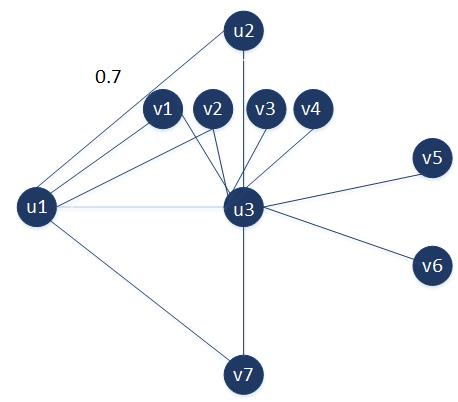
\includegraphics[width=80mm]{common_neighbors.jpg}
	\caption{Ryšių grafo fragmentas} \label{common_neighbors}
\end{figure}

\ref{common_neighbors} pav. pavaizduotas socialinio tinklo fragmentas, kuriame žinomas tik $u_2$ pasitikėjimas $u_1$, kuris šiame pavyzdyje yra lygus $0.7$. Tarkime, kad norime įvertinti $t_{u_3}(u_1)$. Iš grafo matosi, kad $r(u_1)=4$, $r(u_3) = 7$ ir $br(u_1,u_3)=3$ ($u_1$ turi ryšį su 4 naudotojais, $u_1$ - su $7$, o šių naudotojų bendrų ryšių skaičius - $3$). Žinodami, kad $t_{u_2}(u_1) = 0.7$, galime teigti, kad $t_{u_3}(u_1)$ tikrai nebus didesnis nei $t_{u_2}(u_1)$, nes trūkstamas propagavimo kelio pasitikėjimo įvertis $t_{u_3}({u_2})$ nebus didesnis už $1$. Jį galima įvertinti jau minėta taisykle \ref{rule:sim} .
Kitas būdas - spręsti skaitinės prognozės uždavinį. Naudojant mokymo duomenis būtų galima įvertinti sąryšį tarp bendrų ryšių skaičiaus ir pasitikėjimo įverčio. Mokymo duomenys – matrica pavidalo 
\begin{displaymath}
[ \boldsymbol{R_1}, \boldsymbol{R_2}, \boldsymbol{BR}, \boldsymbol{Y}]
\end{displaymath}
Čia 
%\begin{equation}
%\boldsymbol{R_1} = \frac{\verb{ dviejų naudotojų, sujungtų pasitikėjimo ryšiu, bendrų ryšių skaičius }}{\verb{|naudotojo, kuris pasitiki kitu naudotoju ryšių skaičius|}}
%\end{equation}
%ir 
%\begin{equation}
%\boldsymbol{R_2} = \frac{\verb{|dviejų naudotojų, sujungtų pasitikėjimo ryšiu, bendrų ryšių skaičius|}}{\verb{|naudotojo, kuriuo pasitiki kitas naudotojas ryšių skaičius|}}
%\end{equation}
 o $\boldsymbol{Y}$ - priklausomas žinomo pasitikėjimo įverčio tarp jų vektorius. Tyrime, siekiant nustatyti $Y$ priklausomybę nuo $\boldsymbol{R}_1$ ir $\boldsymbol{R}_2$ taikoma tiesinė regresija. Rezultatai pristatyti kitame skyrelyje.
\subsubsection{Rezultatai}
\indent
Metodų efektyvumą sprendžiant šalto starto problemą vienareikšmiškai įvertinti ir palyginti neįmanoma dėl to, kad kiekvienas metodas taikomas skirtingose situacijose. Bendrų kaimynų metodą prasmingiausia taikyti, kai žinomi tik naudotojo ryšiai su kitais naudotojais. Dėl to, kad ši informacija nėra išgaunama iš tikrų reitingų, šio metodo tikslumas gali būti mažesnis negu tradicinio bendradarbiavimo filtravimo.
\newline
\indent
Taikant bendrų kaimynų metodą, yra svarbūs naudotojų ryšių ir bendrų ryšių skaičiai. Buvo sudaryta duomenų matrica pavidalo $[ \boldsymbol{R_1}, \boldsymbol{R_2},  \boldsymbol{Y}]$, kur $\boldsymbol{R_1}$ ir $\boldsymbol{R_2}$ - naudotojų $u_1$ ir $u_2$ bendrų tarpusavio ryšių skaičiaus santykis su naudotojų $u_1$ ir, atitinkamai, $u_2$ ryšių skaičiumi, o $\boldsymbol{Y}$ - prognozuojamas pasitikėjimas. Mokymo imtį sudaro naudotojų $201542$ poros, kurioms duomenų paruošimo etape pavyko įvertinti panašumą ir kurios turi vieną arba daugiau bendrą ryšį. Šiems duomenims pritaikius tiesinę regresiją, gauta tokia formulė:
\begin{equation}\label{eq:CN_all}
y = 0.046 \times r_1 + 0.021 \times r_2 + 0.406
\end{equation}
Akivaizdu, kad koeficientai (rodantys priklausomybę)  yra gana maži - artimi nuliui. Tai rodo, kad pirminė prielaida apie sąryšį tarp pasitikėjimo ir bendrų ryšių skaičiaus - naudotojo ryšių skaičiaus santykio šiems duomenims nepasitvirtino. Tačiau parinkę kitokią naudotojų imtį - tokią, apie kurią turime daugiau informacijos, šiuo atveju su didesniu bendrų ryšių skaičiumi, gauname kiek kitokį vaizdą. Parinkę naudotojų poras, kurios turi daugiau negu 150 bendrų ryšių (tokių yra 634), gauname tokią formulę:
\begin{equation}\label{eq:CN_150}
y = 0.356 \times r_1 + 0.366 \times r_2 + 0.0644
\end{equation}
\newline
Iš tiesų tokia imtis aiškiau leidžia įžvelgti priklausomybę tarp bendrų ryšių. Rezultatai rodo, kad tiek $r_1$, tiek $r_2$ yra vienodai svarbūs.
\indent
\begin{figure}[ht!]
	\centering
	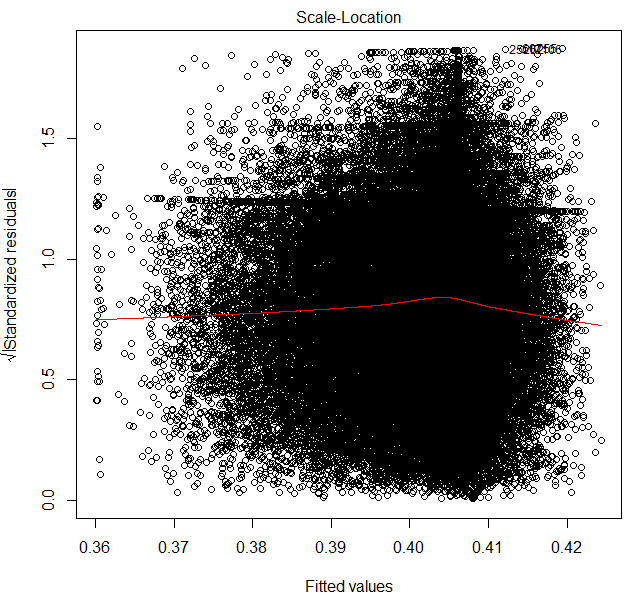
\includegraphics[width=80mm]{CN_residuals.png}
	\caption{Pasitikėjimo prognozių ir standartizuotų liekanų taškinė diagrama} \label{CN_residuals}
\end{figure}
\begin{figure}[ht!]
	\centering
	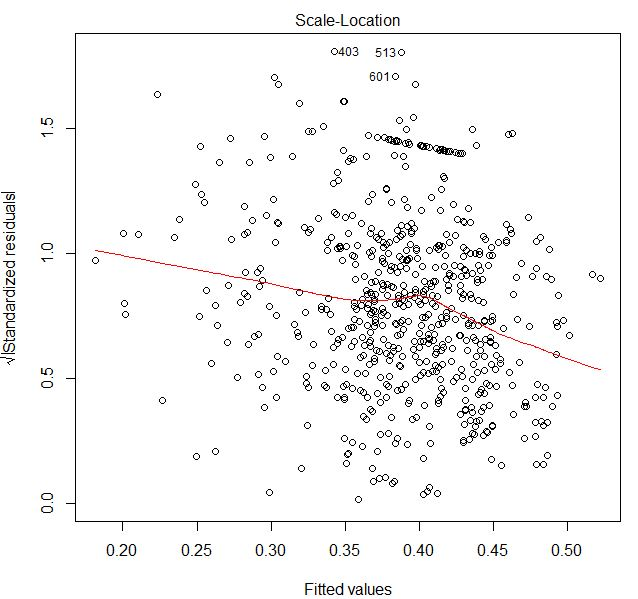
\includegraphics[width=80mm]{CN_residuals_150.jpg}
	\caption{Pasitikėjimo prognozių ir standartizuotų liekanų taškinė diagrama daugiau nei 150 bendrų ryšių turinčioms naudotojų poroms} \label{CN_residuals_150}
\end{figure}
Pav. \ref{CN_residuals} pavaizduotame grafike matosi prognozės ir šaknies iš standartizuotų liekanų taškinė diagrama. Dėl mažų regresijos koeficientų pasitikėjimo prognozės yra išsidėsčiusios mažame intervale, o liekanos - gana didelės. Prognozės tikslumas mažiausias apie vidurkį - tai yra toms naudotojų poroms, kurios turėjo mažą bendrų - savo ryšių skaičiaus santykį, tai yra tiems, apie kuriuos buvo žinoma mažiausiai. Pav. \ref{CN_residuals_150} vaizdas kiek kitoks. Naudotojų poroms, kurioms prognozuotas mažesnis pasitikėjimas pastebimas mažesnis prognozės tikslumas. Kuo mažesnis pasitikėjimas prognozuojamas, tuo yra mažesnis bendrų draugų skaičiaus ir draugų skaičiaus santykis. Kaip ir tikėtasi, prognozė geriausiai veikia naudotojams, kurie turi didžiausias $r_1$ ir $r_2$ reikšmes.
\newline
\indent
Remiantis gautomis formulėmis buvo įvertintas pasitikėjimas, o tuomet pritaikius bendradarbavimo filtravimą, naudojant gautus įverčius, prognozuoti naudotojų įvertinimai. Rezultatai lyginami su rezultatais, gautais taikant bendradarbiavimo filtravimą pradiniams pasitikėjimo duomenims. Imtis - atsitiktinai parinkta 2000 naudotojų aibė. 
\begin{center}
	\captionof{table}{Bendrų kaimynų metodo taikymo rezultatai}
	\begin{tabular}{ | l | l | l | l | }
		\hline
		Metodas taikomas pasitikėjimui rasti & $MAE$ & $MAUE$ & $RMSE$\\ \hline
		Pasitikėjimas (Pyrsono koreliacija)        & 0.902 & 0.913 & 1.167  \\ \hline
		Pasitikėjimo prognozė taikant \ref{eq:CN_all}	  					& 0.913 & 0.905 & 1.182  \\ \hline
		Pasitikėjimo prognozė taikant \ref{eq:CN_150} 					& 0.8900 & 0.91329 & 1.114  \\ \hline
		\hline
	\end{tabular}
\end{center}

Skirtumas tarp $MAE$ ir $RMSE$ rezultatų gautų taikant bendrų kaimynų metodą nuo bazinių rezultatų skiriasi nežymiai. Geriausi rezultatai pagal MAE ir RMSE gauti naudojant prognozę, sudarytą remiantis daugiausiai ryšių turinčių naudotojų imtimi. Šiek tiek didesnis $MAUE$ skirtumas. Taip yra dėl to, kad naudotojai turi nevienodą skaičių reitingų ir $MAUE$ atsižvelgia į tai. Vadinasi, bendrų kaimynų metodas sudarė prognozes mažiau reitingų turėjusiems naudotojams su mažesniu tikslumu negu bazinis bendradarbiavimo filtravimo metodas.
\newline
\indent
Apibendrinant galima pasakyti, kad hipotezė apie pasitikėjimo priklausomybę nuo bendrų ryšių skaičiaus nepasitvirtino. Taip yra dėl to, kad modelis neatsižvelgia į tai, kad daug pasitikėjimo ryšių yra tiesiog atsitiktiniai - vienam naudotojui patiko kito naudotojo nuomonė apie vieną elementą ir jis pažymėjo, kad juo pasitiki. Tačiau galime būti tikri, kad atsiras daug elementų dėl kurių nuomonė nesutaps. Ypač tai aktualu, kai kalbame apie visai kitokius elementus, nei tas, remiantis kuriuo buvo nuspręsta pasitikėti - elementus, priklausančius kitoms kategorijoms.
\subsection{Sričių panašumo metodas}

\subsubsection{Rekomendacinės sistemos su pasitikėjimu kategorijose modeliavimas}
\indent
Šiuo metu nėra tokio duomenų rinkinio, tinkančio atliekamam tyrimui apie RS, kurioje elementai priklauso kategorijoms ir naudotojai išreiškia pasitikėjimą kategorijose. Dėl šios priežasties dalis tyrimo skirta RS modelio sudarymui ir duomenų generavimui. Siekiama sukurti duomenų struktūrą, turinčią tokius elementus:
\begin{itemize}
	\item Kategorijos
	\item Naudotojai
	\item Elementai (reitinguojami produktai) priklausantys kategorijoms
	\item Naudotojo tarpusavio pasitikėjimai kategorijose (tolydi reikšmė tarp 0 ir 1)
	\item Naudotojų reitingai, priskirti elementams
\end{itemize}
Toliau bus aprašyti kiekvieno iš elementų generavimo algoritmai.
\subsubsubsection{Kategorijos}
\indent
Kategojų modeliavimas - pirmas algoritmo žingsnis. Juo siekiama apibrėžti ne tik kategorijas, kurioms gali priklausyti elementai bet ir kiekvieno elemento bruožus bei kiekvieno naudotojo pirmenybes. Dabar generuojami duomenys gali būti vertinami kaip filmų rekomendacinės sistemos duomenys. Apibrėžiame kategorijas:
\begin{itemize}
	\item $X_1$ - drama
	\item $X_2$ - komedija
	\item $X_3$ - siaubo
	\item $X_4$ - trileris
	\item $X_5$ - fantastika
\end{itemize}
Toliau apibrėžiame, kiek kiekviena iš šių kategorijų yra susijusi su kitomis. Heuristiškai sudarome matricą:
\begin{center}
	\captionof{table}{Kategorijų matrica SP1}
	\begin{tabular}{||c c c c c c||} 
		\hline
		Kategorijos & $X_1$ & $X_2$ & $X_3$ & $X_4$ & $X_5$ \\ [0.5ex] 
		\hline\hline
		$x_1$ & 0.55 & 0.2 & 0.2 & 0.2 & 0.3 \\ 
		\hline
		$x_2$ & 0.2 & 0.6 & 0.05 & 0.05 & 0.1 \\
		\hline
		$x_3$ & 0.05 & 0.05 & 0.35 & 0.1 & 0.05 \\
		\hline
		$x_4$ & 0.1 & 0.05 & 0.2 & 0.65 & 0.05 \\
		\hline
		$x_5$ & 0.1 & 0.1 & 0.2 & 0 & 0.5 \\ [1ex] 
		\hline
	\end{tabular}
\end{center}
Čia $X_1, .., X_5$ žymime kategorijas, o $x_1, .., x_5$ kategorijas atitinkančius požymius. Taigi iš šios matricos galime teigti, kad pavyzdžiui:
\begin{itemize}
	\item $X_4$ (trileris) yra gryniausias žanras, tai yra, turintis daugiausiai savo kategoriją atitinkančio požymio (kadangi turi didžiausią matricos įstrižainėje esančią reikšmę)
	\item $X_3$ (siaubo) - mažiausiai gryna kategorija (nes bruožų pasiskirstymas yra tolygiausias)
	\item $X_4$ kategorija neturi $x_5$ bruožo (trileris neturi fantastikos bruožų)
\end{itemize} 
Akivaizdu, kad šie teiginiai yra subjektyvūs. Didesnio objektyvumo galima pasiekti, pavyzdžiui, atliekant apklausas.
\newline
\indent
Atkreipkite dėmesį - tai tik pavyzdys, tyrimo eigoje bus atlikta eksperimentų su RS, kurios bus apibrėžtos kitomis kategorijų matricomis. 
\newline
\indent
Ši matrica bus naudojama generuojant elementus. Nuo to, kokie yra elementai priklauso tai, kaip juos vertina naudotojai, o nuo to priklauso ir tai, kaip naudotojai vertinas vienas kito patikimumą. Taigi, ši matrica - RS duomenų generavimo pagrindas.

\subsubsubsection{Naudotojai}
\indent
Naudotojas apibrėžiamas kaip vektorius $(y_1, y_2, y_3, y_4, y_5, q)$, kur $\sum\limits_{i=1}^{5} y_i = 1$ ir $q\in[0,1]$. $y_1, y_2, y_3, y_4, y_5$ reiškia naudotojo pirmenybes - kiek svarbus jam yra tam tikras bruožas elemente.
$q$ - kokybės parametras rodo, kiek naudotojas yra jautrus elemento kokybei. Kokybės parametro motyvacija tokia - net jei žmogui apskritai nepatinka siaubo filmai, labai tikėtina, kad egzistuoja bent vienas kurį jis vertintų labai gerai (dėl to, kad tas filmas yra aukštos kokybės ir patinka daugumai žmonių). 
\newline
\indent 
Praktiškai algoritmas realizuojamas taip:
\begin{itemize}
	\item sugeneruojame 5 atsitiktinius skaičius tarp 0 ir 1 (naudojant tolygų skirstinį)
	\item randame jų sumą
	\item kiekvienam bruožui priskiriame reikšmę lygią pirmame žingsnyje sugeneruotai reikšmei padalintai iš visų reikšmių sumos
	\item kokybės parametrui priskiriame atsitiktinę reikšmę tarp 0 ir 1
\end{itemize}
Taip užtikriname, kad naudotojai yra tikrai atsitiktiniai ir įvairūs pirmenybių prasme - naudotojui gali patikti tiek siaubo filmai, tiek komedijos, nors tarp šių kategorijų panašumo nėra.
\subsubsubsection{Elementai}
\indent
Elementas apibrėžiamas vektoriumi $(c, z_1, z_2, z_3, z_4, z_5, q)$. Čia $c$ nurodo, kuriai karegorijai priklauso elementas, parametrai $z_1, z_2, z_3, z_4, z_5$ rodo, kiek elementas pasižymi kiekvienu bruožu, o $q$ - kokybės parametras. Generuojant elemntus negalime taikyti tokio paties metodo, kaip naudotojo atveju, nes elementas priklauso vienai kategorijai, o tai reiškia, kad bruožų reikšmės negali būti visiškai atsitiktinės. Jas generuojame pasinaudodami normaliuoju skirstiniu su vidurkiu lygiu reikšmei gautai iš kategorijų matricos, aprašytos skyrelyje apie kategorijas ir parinkta dispersija (tokia, kad duomenys būtų panašūs į realius - parinkus per didelę dispersiją rezultatai gaunasi labai triukšmingi). Vidurkis parenkamas taip: pažiūrėję į $c$ reikšmę atfiltruojame kategoriją (stulpelį). Tada turime vidurkių, naudojamų generuojant $z_1, z_2, z_3, z_4, z_5$, vektorių. Kokybės parametras, kaip ir naudotojo atveju, parenkamas atsitiktinai pagal normalųjį skirstinį su vidurkiu $0.6$ ir dispersija lygia $0.4$. Jei sugeneruota reikšmė didesnė už 1 arba mažesnė už 0, ji priskiriama 1 arba 0 atitinkamai.
\subsubsubsection{Reitingai}
\indent
Naudotojo reitingai elementams generuojami naudojant naudotojo pirmenybes ir reiklumo kokybei parametrą bei atitinkamus produkto parametrus. Siekiama, kad jų pasiskirstymas būtų kuo artimesnis tikrovei, tai jie nebūtų pasiskirstę galimų reikšmių kraštuose ir nebūtų pernelyg vienodi. Sugeneruotų duomenų charakteristikos bus pateiktos kitame skyrelyje. 
\newline
\indent
Kiekvienam naudotojui parenkamas atsitiktinis įvertintų elementų skaičius naudojant atsitiktinį dydį pasiskirsčiusį pagal normalųjį skirstinį su vidurkiu 30 ir dispersija 27. Parinkta didelė dispersija užtikrina, kad duomenys bus artimesni tikriems - Epinions.com duomenų rinkinyje vieno naudotojo įvertintų elementų skaičius svyruoja nuo 0 iki 655. Kiekvienam atsitiktinai parinktam elementui generuojamas reitingas tokiu būdu:
\begin{equation}
r_u(p) = 5 \times ((1-q_u) \sqrt{pos(corr(X_u,Y_p))} + q_u q_p)
\end{equation}
čia
\begin{itemize}
	\item $r_u(p)$ - naudotojo $u$ reitingas elementui $p$
	\item $q_u$ - naudotojo $u$ kokybės reiklumo parametras
	\item $q_p$ - elemento $p$ kokybės parametras
	\item $X_u$ - naudotojo $u$ primenybių rinkinys 
	\item $Y_p$ - elemento $p$ bruožų rinkinys
	\item $pos(x)$ - $f[-1,1] -> [0,1]$
\end{itemize}
\indent
Idealiais atvejais, kai naudotojo reiklumas kokybei ir elemento kokybė lygi 1 arba naudotojo reiklumas kokybei lygus 0, tačiau elemento charakteristikos tobulai atitinka anudotojo pirmenybes, reitingas lygus 5. Tyrimo eigoje pastebėta, kad koreliacijos funkcijos įtaka pernelyg maža, todėl ji padidinama naudojant pasirinktą iškilią funkciją (šiuo atveju šaknis suteikia pageidaujamą efektą).
\subsubsubsection{Pasitikėjimai}
\indent
Pasitikėjimo reikšmės - svarbiausios prognozuojant reitingus, parodančios kokį svorį suteikti patikėtinio nuomonei apie elementą. Šiame tyrime naudotojai vieni kitais pasitiki kategorijos lygmenyje. Buvo išbandyti du pasitikėjimo reikšmių generavimo būdai.
\newline
\indent
Taikant pirmąjį būdą pasitikėjimas tarp dviejų naudotojų tam tikroje kategorijoje generuojamas lyginant naudotojų tarpusavio pirmenybes tos kategorijos atžvilgiu. Taigi pasitikėjimas kategorijoje $X_1$ tarp naudotojų $u(0.1, 0.2, 0.2, 0.5, 0, q_u)$ ir $v(0.2, 0.2, 0.2, 0.2, 0.2, q_v$ randamas taip:
\begin{equation}
t_u(v) = \max(x_1^u, x_1^v) - \min(x_1^u, x_1^v) = 0.2 -0.1 = 0.1
\end{equation}
Tokiu būdu rasti pasitikėjimai tenkina šias savybes:
\begin{itemize}
	\item yra intervale tarp 0 ir 1
	\item nepriklauso nuo kategorijų skaičiaus
\end{itemize}
\indent
Tolimesnis tyrimas parodė, kad šis būdas nėra pakankamai geras. Pagrindinė to priežastis ta, kad vertinant pasitikėjimą tam tikroje kategorijoje naudojamas tik vienas (tą kategoriją atitinkantis) bruožas, o kategorijos savaime nėra vienalytės - jos turi įvairių bruožų, kurie aprašyti kategorijų matricoje. Taigi, jei kategorijų matrica būtų vienetinė - šis būdas veiktų. Remiantis šiuo pastebėjimu buvo išvestas pasitikėjimo interpoliavimo metodas, kuris aprašytas paskutiniame tyrimo skyriuje. 
\newline
\indent
Kitas būdas geresnis - jis, nors ir netiesiogiai, atsižvelgia į kategorijų matricą. Naudotojų, kurie pasitiki vienas kitu, poros ir kategorijos, kurioms generuojamas pasitikėjimas parenkami atsitiktinai, kaip ir anstesnio būdo atveju. Naudotojų porai pasitikėjimas generuojamas taip: parenkami $n$ atsitikinių elementų iš atitinkamos kategorijos ir jiems generuojami abiejų naudotojų reitingai (kaip aprašyta ankstesniame skyrelyje). Turint abiejų naudotojų reitingų vektorius, galime rasti panašumą tarp jų taikant vieną iš panašumo metrikų. Šiuo atveju, taikyta Pyrsono koreliacija. Rastas panašumas transformuojamas taip, kad priklausytų intervalui tarp 0 ir 1, o tada prilygimamas pasitikėjimui. Taikant tokį metodą atsižvelgiama į visas kategorijų charakteristikas. Tai labai svarbu tolimesniam tyrimui, ypač panašumo tarp sričių įvertinimui, kuris nagrinėjamas tolimesniuose skyriuose.
\subsubsubsection{Sugeneruoto duomenų rinkinio charakteristikos }
\indent
Norint iliustruoti tam tikrus teigius apie taikytus metodu, praverčia duomenų rinkiniai su skirtingomis chrakteristikomis. Pavyzdžiui, norėdami parodyti propagavimo metodų efektyvumą kitame skyriuje, pravers duomenų rinkinys su mažai duomenų apie pasitikėjimą (tai yra naudotojai turės mažai patikėtinių). Tam, kad būtų aišku, koks duomenų rinkinys naudotas konkrečiu atvejus, bus pateikta rinkinį apibūdinanti generavimo parametrų lentelė. 
%parametrai - useriu skaicius, ju pasitikejimo rysiu skaiciaus skirstinys, ju ivertintu produktu skaiciaus skirstiny, produktu skaicius, kiek bendru elementu iverinama norint rasti pasitikejima, koks propagavimo metodas naudojamas, kokia sriciu panasumo matrica naudojama%
\begin{center}
	\begin{tabular}{||c c||} 
		
		
		Elementų skaičius & 300 \\
		Naudotojų skaičius & 100 \\
		Naudotojo ryšių skaičiaus pasiskirstymas &  N(10, 9) \\
		Naudotojo įvertintų elementų skaičiaus pasiskirstymas & N(30,27) \\
		Vertinamas bendrų elementų skaičius ieškant pasitikėjimo & 12 \\
		Propagavimo metodas & Vidurkio\\
		Kategorijų matrica & SP1 \\
	\end{tabular}
	
\end{center}
\subsubsection{Metodas}
\indent
Šalto starto sąvoka nėra vienareikšmiškai apibrėžiama - negalime iš anksto žinoti, kiek ir kokių reikia duomenų, kad situacija tenkintų apibrėžimą ir taikomas metodas veiktų kaip tikimąsi. Aplinkoje, apie kurią dabar rašoma, naudotojas gali būti šalto starto padėtyje, kai kalbame apie vieną sritį, tačiau kitoje srityje padėtis gali būti priešinga. Kitaip tariant, jeigu norime sužinoti, koks yra $t_u^2(v)$, ir žinome, kad naudotojo $u$ pasitikėjimo naudotoju $v$ srityje $T_1$ lygis yra $0.8$, o sričių $T_1$ ir $T_2$ panašumas $sim(T_1, T_2) = 0.9$, nieko nežinodami apie naudotojų santykį $T_2$ klausimu, galime įvertinti jų tarpusavio pasitikėjimą tiesiog padauginę žinomos srities pasitikėjimo įvertį iš sričių tarpusavio panašumo įverčio.
\newline
\indent
Ši idėja yra pritaikoma ne tik šalto starto atveju, kai kalbama apie naudotoją, bet ir naujos srities šalto starto atveju. Socialinius tinklus pagal pasitikėjimo sričių daugialypiškumą galima išskirti į du tipus:
\begin{itemize}
	\item daugiaprofilinius - juose galimos įvairios pasitikėjimo sritys - tokios, kurias galima surikiuoti pagal panašumą ir tarp pirmos bei paskutinės nėra jokio panašumo.
	\item specializuotos - juose pasitikėjimo sritys yra gana artimos. Tokio tinklo pavyzdys galėtų būti kino mėgėjų socialinis tinklas, o sritys - įvairūs žanrai.
\end{itemize}

Siūlomas metodas geriau veikia antrojo tipo atveju, kai sritys yra tarpuavyje panašios. Kai sritys pernelyg skirtingos, o panašumas mažas - panaudoti informaciją apie panašumą yra sudėtinga.
\begin{figure}[ht!]
	\centering
	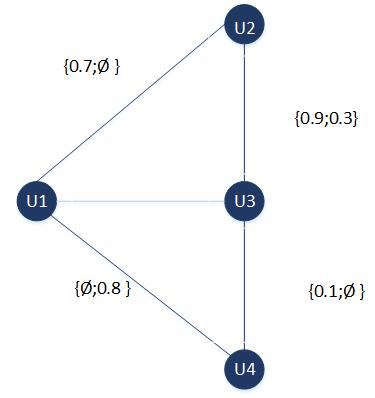
\includegraphics[width=60mm]{multiarea.jpg}
	\caption{Ryšių grafo fragmentas} \label{multiarea}
\end{figure}
Tarkime, kad turime situaciją pavaizduotą grafe \ref{multiarea}, kuriame pateikti naudotojų tarpusavio pasitikėjimai ${t_1, t_2}$, ir norime žinoti, kiek $u_1$ pasitiki $v$ dėl $T_2$. Tiesioginio būdo nėra, nes abiejuoe galimuose keliuose - $u_1 - u_2 - v$ ir $u_1 - u_4 - v$ yra trūkstamų duomenų - pirmu atveju nežinome $t_{u_1}^2(u_2)$, antru - $t_{u_4}^2(v)$, tačiau matome, kad egzistuoja kelias $u_1 - u_2 - v$, pagal kurį galime įvertinti $t_{u_1}^1(v)$
\begin{displaymath}
t_{u_1}^1(v)=t_{u_1}^1(u_2) \times t_{u_2}^1(v) = 0.7 \times 0.9 = 0.63
\end{displaymath}
Žinodami, kad sričių panašumas $s^d(T_1, T_2) = 0.9$, gauname
\begin{displaymath}
t_{u_1}^1(v)=t_{u_1}^1(v) \times s^d(T_1, T_2) = 0.63 \times 0.9 = 0.6048
\end{displaymath}
\indent
Šį metodą galima taikyti dviem būdais:
\begin{itemize}
	\item globaliai - panašumai tarp sričių randami visai sistemai.
	\item naudotojo lygmeniu - turint sukaupus daugiau duomenų apie naudotoją galima vertinti jo asmeninį sričių panašumo suvokimą.
\end{itemize}
\indent Norėdami įvertinti panašumą tarp sričių turime turėti naudotojų porų ir jų tarpusavio pasitikėjimo pagal sritis sąrašą. Tada panašumą tarp sričių galime įvertinti taikydami vieną iš panašumo radimo metodų (Pyrsono, Spearmano koreliacija, kosinuso panašumas) turimiems pasitikėjimo (arba panašumo) duomenims. 
\newline
\indent Kitas būdas, remiantis kuriuo galime rasti panašumą tarp sričių - ieškoti panašumo tarp sričių charakteristikų iš kategorijų matricos. Tiesa, šis būdas veikia tik vertinant sričių panašumą visoje sistemoje.
\newline
\indent 
Tarkime, kad žinome panašumą tarp sričių. Belieka atsakyti į klausimą - kaip ši informacija gali padėti įvertinti pasitikėjimą tarp naudotojų. Tyrime bus išbandyti du metodai:
\begin{itemize}
	\item MAXDS metodas. Tarkime, kad turime naudotojų porą su žinomais pasitikėjimais dviejose srityse ir nežinomais trijose. Norėdami įvertinti nežinomus pasitikėjimus, parenkame tą žinomą pasitikėjimo reikšmę, kuri yra didžiausia ir naudodami ją kaip pagrindą, nežinomas randame sudauginę ją su atitinkamos kategorijos panašumu. Šio metodo trūkumas tas, kad atsižvelgiama ne į visą žinomą infromaciją. 
	\item AVGDS metodu siekiama panaudoti visą žinomą informaciją. Nežinomos pasitikėjimo reikšmės randamos ieškant randant žinomų pasitikėjimų sudaugintų su sričių panašumu vidurkį su svoriais. Svoriai šioje formulėje - tie patys vidurkiai.
	\begin{equation}
		t_u^{T_i}(v) = \frac{\sum\limits_{j \in T } t_u^{T_j}(v) \times sim(T_i, T_j)^2}{\sum\limits_{j \in T} sim(T_i, T_j)}
	\end{equation}
\end{itemize}
\subsubsubsection{Pasitikėjimų pagrįstų RS metodai}

\indent
Kai kalbama apie rekomendacines sistemas su socialinių tinklų duomenimis daugiausia tyrimų [kokių] atlikta nagrinėjant agregavimo ir propagavimo metodus, kurie remiasi prielaida apie pasitikėjimo tranzityvumą. Šio tyrimo kontekste į šiuos metodus galima žiūrėti kaip į tam tikrą duomenų papildymo būdą prieš taikant sričių panašumo metodą. 
\indent 
Tyrime bus išbandyti keli trumpiausio kelio šeimos algoritmai. Trumpiausio kelio algoritmas randa trumpiausią kelią tarp dviejų naudotojų ir randa pasitikėjimą tarp jų vienu iš šių operacijų pasitikėjimo įverčiams, esančiams pasitikėjimo kelyje:

	\begin{itemize}
		\item daugyba - SHORTMULTI
		\item aritmetinis vidurkis - SHORTARI
		\item harmoninis vidurkis - SHORTHARM
	\end{itemize}
\subsubsection{Rezultatai}
Šiuo eksperimentu siekiama ištirti sričių panašumo metodo efektyvumą. Tačiau be šio galutinio tikslo, taip pat galima paminėti ir tarpinius tikslus - išbandyti duomenų rinkinio generavimo algoritmą ir kitų žinomų metodų, naudojamų pasitikėjimų radimui, efektyvumą.
\newline
\indent
Eksperimentas atliktas naudojant du skirtingus generuotus duomenų rinkinius. Pirmas - duomenų rinkinys, aprašytas ankstesniame skyriuje. Jis pasižymi tuo, kad kategorijos yra gana skirtingos ir sričių panašumas yra mažas. Kitas duomenų rinkinys bus generuojamas naudojant kategorijų matricą, kurioje sritys yra tarpusavyje panašios. 
\subsubsubsection{Eksperimentas naudojant RS su skirtingomis kategorijomis}
Ankstesniame skyrelyje sugeneruoto duomenų rinkinio charakteristikos yra tokios:
\begin{center}
	\begin{tabular}{||c c||} 
		Naudotojų, įvertinusių bent vieną elementą, skaičius & 87 \\
		Šalto starto naudotojų skaičius & 18 \\
		Ryžtingų naudotojų skaičius  & 6 \\
		Reitingų standatinis nuokrypis & 1.5 \\
	\end{tabular}
\end{center}
Reitingų pasiskirstymas:
\begin{center}
	\begin{tabular}{||c c c c c||} 
		1 & 2 & 3 & 4 & 5 \\
		612 & 345 & 370 & 730 & 839 \\
	\end{tabular}
\end{center}
\indent
Šiam duomenų rinkiniui pagal nustatytus vertinimo kriterijus gauname tokius rezulatus:
\begin{center}
	\captionof{table}{BF rezultatai taikomi RS duomenims}
	\begin{tabular}{||c c c c c c c ||} 
		Duomenų rinkinio poaibis & Naudotojų skaičius & MAE & MAUE & RMSE & RC & UC \\
		\hline
		Visi naudotojai & 87 & 1.04 & 0.98 & 1.5 & 0.22 & 0.65 \\
		\hline
		Šalto starto naudotojai & 19 & - & - & - & 0 & 0 \\
		\hline
		Ryžtingi naudotojai & 6 & 1.17 & 1.17 & 1.84 & 0.06 & 0.17 \\
	\end{tabular}
\end{center}
%\subsubsubsubsection{Pasitikėjimo propagavimas ir agregavimas}
\indent
Tokiems duomenims galime taikyti globalaus sričių panašumo metodą. Išbandyti AVGDS (sričių panašumo vidurkio) ir MAXDS (sričių panašumo maksimumo) metodai.
\begin{center}
	\captionof{table}{BF + AVGDS rezultatai taikomi RS duomenims}
	\begin{tabular}{||c c c c c c c ||} 
		Duomenų rinkinio poaibis & Naudotojų skaičius & MAE & MAUE & RMSE & RC & UC \\
		\hline
		Visi naudotojai & 87 & 1.04 & 0.98 & 1.49 & 0.33 & 0.69 \\
		\hline
		Šalto starto naudotojai & 19 & - & - & - & 0 & 0 \\
		\hline
		Ryžtingi naudotojai & 6 & 0.96 & 0.67 & 1.43 & 0.11 & 0.5 \\
	\end{tabular}
\end{center}

\begin{center}
	\captionof{table}{BF + MAXDS rezultatai taikomi RS duomenims}
	\begin{tabular}{||c c c c c c c ||} 
		Duomenų rinkinio poaibis & Naudotojų skaičius & MAE & MAUE & RMSE & RC & UC \\
		\hline
		Visi naudotojai & 87 & 1.03 & 0.95 & 1.46 & 0.33 & 0.69 \\
		\hline
		Šalto starto naudotojai & 19 & - & - & - & 0 & 0 \\
		\hline
		Ryžtingi naudotojai & 6 & 1.03 & 0.69 & 1.59 & 0.11 & 0.5 \\
	\end{tabular}
\end{center}
\indent
Iš rezultatų matosi, kad tiek tikslumas, tiek padengimas pagerėjo visų naudotojų imčiai. Didelis tikslumo padidėjimas ryžtingų naudotojų atveju  iš dalies gali būti paaiškintas atsitiktinumu dėl mažos imties, tačiau atlikus daugiau eksperimentų pastebėta, kad tikslumas beveik visada nežymiai keičiasi į gerąja pusę, o reitingų padengimas didėja vidutiniškai apie 50\% kiekvienai imčiai.  \ref{BASEDS} pav. matosi, kaip atrodo ryšių grafas po sričių panašumo metodo pritaikymo.
\begin{figure}[ht!]
	\centering
	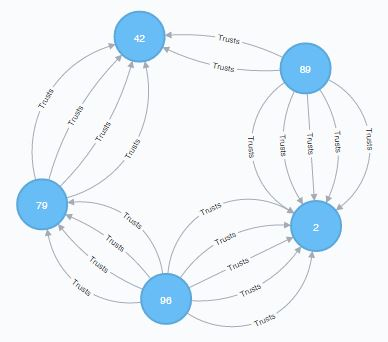
\includegraphics[width=80mm]{BASEDS.jpg}
	\caption{Ryšių grafo fragmentas pritaikius sričių panašumo metodą} \label{BASEDS}
\end{figure}
\newline
\indent
Nepastebėta reikšmingo skirtumo tarp MAXDS ir AVGDS metodų, dėl to toliau  bus taikomas tik AVGDS metodas (nes jis atsižvelgia į daugiau informacijos).
\indent  Sričių panašumo metodas nekuria naujų ryšių tarp naudotojų, kurie nieko vienas apie kitą nežino - tą daro kiti metodai, taikantys propagavimo ir agregavimo operatorius. Tačiau šiuos du metodų tipus galima kombinuoti ir taikyti kartu.
\indent
Šis duomenų rinkinys buvo sugeneruotas parinkus tokius parametrus, kad jame egzistuotų duomenų retumo problema. Tai matome iš nedidelių $RC$ ir $UC$ reikšmių. Egzistuojantis problemos sprendimo būdas - taikyti metodus, vertinančius naudotojų tarpusavio pasitikėjimą. Tam pačiam duomenų rinkiniui išbandyti trys trumpiausio kelio metodai, aprašyti ankstesniame skyrelyje (SHORTMULTI, SHORTARI, SHORTGEO). Siekiant vertinti tik svarbias pasitikėjimo reikšmes, nustatmome slenkstį lygų $0.9$, nuo kurio saugosime rastus pasitikėjimus.
\begin{center}
	\captionof{table}{BF + SHORTMULTI rezultatai taikomi RS duomenims}
	\begin{tabular}{||c c c c c c||} 
		Duomenų rinkinio poaibis & MAE & MAUE & RMSE & RC & UC \\
		\hline
		Visi naudotojai & 1.05 & 0.99 & 1.62 & 0.51 & 0.87 \\
		\hline
		Šalto starto naudotojai & 1 & 0.83 & 1.55 & 0.23 & 0.55 \\
		\hline
		Ryžtingi naudotojai & 1.06 & 1.03 & 1.75 & 0.55 & 1 \\
	\end{tabular}
\end{center}

\begin{center}
	\captionof{table}{BF + SHORTARI rezultatai taikomi RS duomenims}
	\begin{tabular}{||c c c c c c||} 
		Duomenų rinkinio poaibis & MAE & MAUE & RMSE & RC & UC \\
		\hline
		Visi naudotojai & 1.15 & 1.09 & 1.88 & 0.65 & 0.92 \\
		\hline
		Šalto starto naudotojai & 1.10 & 1.04 & 1.81 & 0.35 & 0.67 \\
		\hline
		Ryžtingi naudotojai & 1.27 & 1.31 & 2.33 & 0.65 & 1 \\
	\end{tabular}
	
\end{center}

Naudojant geometrinį vidurkį kaip propagavimo operatorių parenkame kitokį slenkstį - $0.6$. 
\begin{center}
	\captionof{table}{BF + SHORTGEO rezultatai taikomi RS duomenims}
	\begin{tabular}{||c c c c c c||} 
		Duomenų rinkinio poaibis & MAE & MAUE & RMSE & RC & UC \\
		\hline
		Visi naudotojai & 1.16 & 1.14 & 1.84 & 0.8 & 0.98 \\
		\hline
		Šalto starto naudotojai & 1.16 & 1.1 & 1.88 & 0.52 & 0.89 \\
		\hline
		Ryžtingi naudotojai & 1.27 & 1.30 & 2.27 & 0.78 & 1 \\
	\end{tabular}
\end{center}
\indent
Atlikus eksperimentus paaiškėjo, kad geriausiai turimiems duomenims veikia SHORTMULTI metodas. Tai paaiškinama tuo, kad jis atsižvelgia į pasitkėjimo mažėjimą (angl. trust decay) esant ilgesniems pasitikėjimo keliams. SHORTARI ir SHORTGEO labiau padidina padengimą, tačiau tikslumas sumažėja pernelyg smarkiai, kad šie metodai būtų vertingi praktikoje.
%Kazka matome is situ rezultatu
%\subsubsubsubsection{Sričių panašumas}
\indent
Kaip minėta anskčiau, sričių panašumo metodas gali būti taikomas nepriklausomai nuo metodų, prognozuojančių naudotojų tarpusavio pasitikėjimą naudojant propagavimo ir agregavimo opetarorius. Jau parodyta, kaip globalus sričių panašumas veikia su baziniais RS duomenimis. Dabar bus siekiama ištirti, kaip veikia sričių panašumo ir agregavimo bei propagavimo metodų kombinacija. Jau parodyta, kad geriausiai iš tiriamų agregavimo ir propagavimo metodų veikia SHORTMULTI metodas, todėl toliau bus tiriamos trys kombinacijos:
\begin{itemize}
	\item  SHORTMULTI + GDS (Pyrsono). Naudojamas globalus sričių panašumas randant Pyrsono koreliaciją tarp pasitikėjimo reikšmių atitinkamoms sritims. Sričių panašumo reikšmės pateiktos \ref{DS1panasumai} lentelėje.
	\item  SHORTMULTI + GDS (sričių charakteristikų). Naudojamas globalus sričių panašumas randant koreliacijas tarp sričių charakteristikų apibrėžtų kategorijų matricoje. Sričių panašumo reikšmės pateiktos \ref{DS1koreliacijos} lentelėje.
	\item  SHORTMULTI + UDS. Sričių panašumas randamas kiekvienam naudotojui ir jo pasitikėjimai išskaičiuojami naudojant jo asmeninį sričių panašumo suvokimą.
\end{itemize}


\begin{center}
	\captionof{table}{Sričių panašumo matrica}
	\begin{tabular}{||c c c c c c||} 
		\hline
		Kategorijos & $X_1$ & $X_2$ & $X_3$ & $X_4$ & $X_5$ \\ [0.5ex] 
		\hline\hline
		$X_1$ & 1 & 0.62 & 0.37 & 0.48 & 0.63 \\ 
		\hline
		$X_2$ & 0.62 & 1 & 0.08 & 0.31 & 0.43 \\
		\hline
		$X_3$ & 0.37 & 0.08 & 1 & 0.53 & 0.45 \\
		\hline
		$X_4$ & 0.48 & 0.30 & 0.53 & 1 & 0.26 \\
		\hline
		$X_5$ & 0.63 & 0.43 & 0.46 & 0.26 & 1 \\ [1ex] 
		\hline
	\end{tabular}\label{DS1panasumai}
\end{center}
\begin{center}
	\captionof{table}{Panašumo tarp kategorijų matrica}
	\begin{tabular}{||c c c c c c||} 
		\hline
		Kategorijos & $X_1$ & $X_2$ & $X_3$ & $X_4$ & $X_5$ \\ [0.5ex] 
		\hline\hline
		$X_1$ & 1 & 0.77 & 0.8 & 0.32 & 0.56 \\ 
		\hline
		$X_2$ & 0.78 & 1 & 0.77 & 0.24 & 0.43 \\
		\hline
		$X_3$ & 0.88 & 0.77 & 1 & 0.35 & 0.56 \\
		\hline
		$X_4$ & 0.32 & 0.24 & 0.35 & 1 & 0.47 \\
		\hline
		$X_5$ & 0.56 & 0.43 & 0.6 & 0.47 & 1 \\ [1ex] 
		\hline
	\end{tabular}\label{DS1koreliacijos}
\end{center}
\indent
Naudojant \ref{DS1panasumai} panašumo matricą trūkstamai informacijai apie pasitikėjimą užpildyti ir naudojant pasitikėjimo slenkstį 0.6 gaunami tokie rezultatai.
\begin{center}
		\captionof{table}{BF + sričių panašumo, gauto naudojant kategorijų matricą, rezultatai taikomi RS duomenims}
	\begin{tabular}{||c c c c c c||} 
		Duomenų rinkinio poaibis & MAE & MAUE & RMSE & RC & UC \\
		\hline
		Visi naudotojai & 1.17 & 1.12 & 1.95 & 0.61 & 0.89 \\
		\hline
		Šalto starto naudotojai & 1.08 & 1.06 & 1.69 & 0.35 & 0.61 \\
		\hline
		Ryžtingi naudotojai & 1.16 & 1.13 & 2 & 0.76 & 1 \\
	\end{tabular}
\end{center}
\indent 
Naudojant \ref{DS1koreliacijos} panašumo matricą trūkstamai informacijai apie pasitikėjimą užpildyti kartu su pasitkėjimo slenksčiu lygiu 0.6 gaunami tokie rezultatai.
\begin{center}
	\captionof{table}{SHORTMULTI + sričių panašumo, gauto naudojant kategorijų matricą, su slenksčiu 0.6, rezultatai taikomi RS duomenims}
	\begin{tabular}{||c c c c c c||} 
		Duomenų rinkinio poaibis & MAE & MAUE & RMSE & RC & UC \\
		\hline
		Visi naudotojai & 1.07 & 0.96 & 1.56 & 0.55 & 0.87 \\
		\hline
		Šalto starto naudotojai & 1.02 & 1.05 & 1.79 & 0.3 & 0.56 \\
		\hline
		Ryžtingi naudotojai & 1.09 & 1.02 & 1.67 & 0.54 & UC \\
	\end{tabular}
\end{center}
\begin{center}
	\captionof{table}{SHORTMULTI + sričių panašumo, gauto naudojant kategorijų matricą, su slenksčiu 0.3, rezultatai taikomi RS duomenims}
	\begin{tabular}{||c c c c c c||} 
		Duomenų rinkinio poaibis & MAE & MAUE & RMSE & RC & UC \\
		\hline
		Visi naudotojai & 1.12 & 1.12 & 1.8 & 0.76 & 0.88 \\
		\hline
		Šalto starto naudotojai & 1.07 & 1.12 & 1.72 & 0.57 & 0.61 \\
		\hline
		Ryžtingi naudotojai & 1.13 & 1.12 & 1.95 & 0.9 & 1 \\
	\end{tabular}
\end{center}
Pastebime, kad turint tokias panašumo reikšmes slenskčio reikšmė lygi 0.6 yra labai didelė - iš tiesų taikydami šį metodą papildomos informacijos galime gauti tik apie $X_1$ ir $X_2$ bei $X_1$ ir $X_5$ kategorijų panašumus (nes tik jų sandauga su žinomu pasitikėjimu, mažesniu už 1, gali viršyti 0.6). Metodas taip pat buvo išbandytas su slenksčiu lygiu 0.3. Nors padengimas ir padidėjo, tačiau tikslumas sumažėjo atitinkamai. 
\newline
\indent 
Paskutinis metodas, kuris bus išbandytas su šiuo duomenų rinkiniu - sričių panašumo naudotojo lygmenyje. Kiekvienam naudotojui rasime jo asmeninę sričių panašumo matricą.
\begin{center}
	\captionof{table}{SHORTMULTI + UDS, su slenksčiu 0.6, rezultatai taikomi RS duomenims}
	\begin{tabular}{||c c c c c c||} 
		Duomenų rinkinio poaibis & MAE & MAUE & RMSE & RC & UC \\
		\hline
		Visi naudotojai & 1.15 & 1.05 & 1.91 & 0.59 & 0.87 \\
		\hline
		Šalto starto naudotojai & 1.10 & 0.86 & 1.88 & 0.24 & 0.56 \\
		\hline
		Ryžtingi naudotojai & 1.14 & 1.12 & 1.95 & 0.9 & 1 \\
	\end{tabular}
\end{center}
\indent
Šio metodo rezultatai ne tokie geri, kaip būtų galima tikėtis - šalto startp naudotojams tiek padengimas, tiek tikslumas gaaunamas geresnis taikant globalų sričių panašumą. Tai galima paaiškinti tuo, kad ieškant naudotojo asmeninio sričių panašumo atsižvelgiama į per mažai duomenų ir dėl to vertinimas būna labiau atsitiktinis. 
\newline
\indent 
Sunku vertinti gautus rezultatus vienareikšmiškai, nes jie susideda iš kelių dydžių. Vis dėlto, vertinant rezultatus, gautus taikant sričių panašumo metodą, reikia pasakyti, kad geriausi rezultatai gauti naudojant sričių panašumus išskaičiuotus iš kategorijų matricos. Viena vertus, tai reiškia, kad kiti metodai, kuriuos galima būtų pritaikyti realiems duomenims - (tiek globalus, tiek naudotojo lygmens), neveikia taip gerai kaip galėtų. Iš kitos pusės, tai įrodo, kad parinkus tinkamas panašumo reikšmes galima išgauti gerų rezultatų siekiant išspręsti duomenų retumo problemą.
\subsubsubsection{Eksperimentas naudojant RS su panašiomis kategorijomis}
\indent 
Analogiškas eksperimentas buvo atliktas kitokiai RS, kurioje kategorijos yra panašios. Šiame skyriuje naudojamas duomenų rinkinys apibrėžiamas paramtetru rinkiniu [] ir kategorijų matrica [SP2].
\begin{center}
	\captionof{table}{RS duomenų rinkinio generavimo parametrai}
	\begin{tabular}{||c c||} 
		
		
		Elementų skaičius & 300 \\
		Naudotojų skaičius & 100 \\
		Naudotojo ryšių skaičiaus pasiskirstymas &  N(10, 9) \\
		Naudotojo įvertintų elementų skaičiaus pasiskirstymas & N(30,27) \\
		Vertinamas bendrų elementų skaičius ieškant pasitikėjimo & 12 \\
		Propagavimo metodas & Vidurkio\\
		Kategorijų matrica & SP1 \\
	\end{tabular}
	
\end{center}
\begin{center}
	\captionof{table}{Kategorijų matrica SP2}
	\begin{tabular}{||c c c c c c||} 
		\hline
		Kategorijos & $X_1$ & $X_2$ & $X_3$ & $X_4$ & $X_5$ \\ [0.5ex] 
		\hline\hline
		$x_1$ & 0.6 & 0.5 & 0.4 & 0.6 & 0.3 \\ 
		\hline
		$x_2$ & 0.2 & 0.1 & 0.2 & 0 & 0.3 \\
		\hline
		$x_3$ & 0.1 & 0.1 & 0.1 & 0.1 & 0.1 \\
		\hline
		$x_4$ & 0.1 & 0.1 & 0.1 & 0.2 & 0.1 \\
		\hline
		$x_5$ & 0 & 0.1 & 0.2 & 0.1 & 0.2 \\ [1ex] 
		\hline
	\end{tabular}\label{DS2}
\end{center}
Sugeneruoto duomenų rinkinio \ref{DS2} charakteristikos yra tokios:
\begin{center}
	\begin{tabular}{||c c||} 
		Naudotojų, įvertinusių bent vieną elementą, skaičius & 87 \\
		Šalto starto naudotojų skaičius & 18 \\
		Ryžtingų naudotojų skaičius  & 6 \\
		Reitingų standatinis nuokrypis & 1.47 \\
	\end{tabular}
\end{center}
Reitingų pasiskirstymas:
\begin{center}
	\begin{tabular}{||c c c c c||} 
		1 & 2 & 3 & 4 & 5 \\
		532 & 339 & 373 & 786 & 849 \\
	\end{tabular}
\end{center}
\indent
Šiam duomenų rinkiniui pagal nustatytus vertinimo kriterijus gauname tokius rezulatus:
\begin{center}
	\captionof{table}{BF rezultatai taikomi RS duomenims}
	\begin{tabular}{||c c c c c c||} 
		Duomenų rinkinio poaibis & MAE & MAUE & RMSE & RC & UC \\
		\hline
		Visi naudotojai & 1.04 & 0.91 & 1.51 & 0.21 & 0.63 \\
		\hline
		Šalto starto naudotojai & - & - & - & 0 & 0 \\
		\hline
		Ryžtingi naudotojai & 1.41 & 1.41 & 2.40 & 0.09 & 0.17 \\
		
	\end{tabular}
\end{center}
\indent
Pritaikius GDS su slenksčiu 0.3 baziniams duomenims gauname tokius rezultatus
\begin{center}
	\captionof{table}{BF rezultatai taikomi RS duomenims}
	\begin{tabular}{||c c c c c c||} 
		Duomenų rinkinio poaibis & MAE & MAUE & RMSE & RC & UC \\
		\hline
		Visi naudotojai & 1.07 & 1 & 1.57 & 0.34 & 0.69 \\
		\hline
		Šalto starto naudotojai & - & - & - & 0 & 0 \\
		\hline
		Ryžtingi naudotojai & 1.30 & 1.30 & 2.23 & 0.14 & 0.17 \\
		
	\end{tabular}
\end{center}
Vėl matome, kad padengimui padidėjus, tikslumas šiek tiek sumažėja. Metodas prie 743 sistemoje esančių originalių pasitikėjimų, pridėjo dar 590 esamiems vartotojams.
\newline
\indent
Iš ansktesnio skyrelio jau aišku, kad iš tiriamų propagavimo ir agregavimo metodų geriausiai veikia SHORTMULTI metodas. Šiam duomenų rinkiniui šio metodo rezultatai panašūs. Kur kas įdomesni rezultatai gauti taikant SHORTMULTI metodą duomenų rinkiniu, kuriam jau buvo pritaikytas sričių panašumo metodas. 
\begin{center}
	\captionof{table}{GDS + SHORTMULTI rezultatai taikomi RS duomenims}
	\begin{tabular}{||c c c c c c||} 
		Duomenų rinkinio poaibis & MAE & MAUE & RMSE & RC & UC \\
		\hline
		Visi naudotojai & 0.97 & 0.86 & 1.40 & 0.34 & 0.85 \\
		\hline
		Šalto starto naudotojai & 0.76 & 0.68 & 0.95 & 0.15 & 0.55 \\
		\hline
		Ryžtingi naudotojai & 0.96 & 0.4 & 1.61 & 0.38 & 0.67 \\
	\end{tabular}
\end{center}
Matome, kad SHORTMULTI metodas taikomas po to, kai buvo pritaikytas sričių panašumo metodas duoda daug geresnį tikslumą ir ne prastesnį padengimą nei kitais atvejais. Dar labiau jį galima padidinti vėl pritaikius sričių panašumo metodą. Gaunamas kiek prastesnis tikslumas, tačiau reitingų padengimas dar labiau padidėjo.
\begin{center}
	\captionof{table}{GDS + SHORTMULTI + GDS rezultatai taikomi RS duomenims}
	\begin{tabular}{||c c c c c c||} 
		Duomenų rinkinio poaibis & MAE & MAUE & RMSE & RC & UC \\
		\hline
		Visi naudotojai & 1.02 & 0.97 & 1.40 & 1.51 & 0.85 \\
		\hline
		Šalto starto naudotojai & 1 & 0.89 & 1.54 & 0.24 & 0.55 \\
		\hline
		Ryžtingi naudotojai & 0.98 & 0.87 & 1.68 & 0.51 & 0.67 \\
	\end{tabular}
\end{center}


\begin{center}
	\captionof{table}{Panašumo tarp kategorijų matrica }
	\begin{tabular}{||c c c c c c||} 
		\hline
		Kategorijos & $X_1$ & $X_2$ & $X_3$ & $X_4$ & $X_5$ \\ [0.5ex] 
		\hline\hline
		$X_1$ & 1 & 0.62 & 0.37 & 0.48 & 0.63 \\ 
		\hline
		$X_2$ & 0.62 & 1 & 0.08 & 0.31 & 0.43 \\
		\hline
		$X_3$ & 0.37 & 0.08 & 1 & 0.53 & 0.45 \\
		\hline
		$X_4$ & 0.48 & 0.30 & 0.53 & 1 & 0.26 \\
		\hline
		$X_5$ & 0.63 & 0.43 & 0.46 & 0.26 & 1 \\ [1ex] 
		\hline
	\end{tabular}
\end{center}
Naudojant tokią panašumo matricą trūkstamai informacijai apie pasitikėjimą užpildyti gaunami tokie rezultatai.
\begin{center}
	\captionof{table}{BF + sričių panašumo, gauto naudojant kategorijų matricą, rezultatai taikomi RS duomenims}
	\begin{tabular}{||c c c c c c||} 
		Duomenų rinkinio poaibis & MAE & MAUE & RMSE & RC & UC \\
		\hline
		Visi naudotojai & MAE & MAUE & RMSE & RC & UC \\
		\hline
		Šalto starto naudotojai & MAE & MAUE & RMSE & RC & UC \\
		\hline
		Ryžtingi naudotojai & MAE & MAUE & RMSE & RC & UC \\
	\end{tabular}
\end{center}
\indent 
Kitokie rezultatai gaunami naudojant sričių panašumo metodą kartu su kitais metodais, naudojančiais socialinių tinklų duomenis. Anskčiau buvo parodyta, kad geriausi rezultatai gauti taikant SHORTGEO metodą. Papildžius šį metodą sričių panašumo metodu gaunami tokie rezultatai.
\begin{center}
	\captionof{table}{BF + SHORTGEO + sričių panašumo, gauto naudojant kategorijų matricą, rezultatai taikomi RS duomenims}
	\begin{tabular}{||c c c c c c||} 
		Duomenų rinkinio poaibis & MAE & MAUE & RMSE & RC & UC \\
		\hline
		Visi naudotojai & MAE & MAUE & RMSE & RC & UC \\
		\hline
		Šalto starto naudotojai & MAE & MAUE & RMSE & RC & UC \\
		\hline
		Ryžtingi naudotojai & MAE & MAUE & RMSE & RC & UC \\
	\end{tabular}
\end{center}



\subsubsubsection{Eksperimento rezultatų taikytų dviem duomenų rinkiniams palyginimas}

\subsection{Problemos ir iššūkiai}
\indent
Didžiausia problema šio tyrimo srityje yra realių duomenų nebuvimas ir negalėjimas praktiškai įvertinti šių metodų tinkamumo. Nėra žinomo socialinio tinklo, kuriame naudotojai išreikštų pasitikėjimą vienas kitu tolydžioje skalėje ir pasitikėjimai galėtų būtų priskirti skirtingose kategorijose. Artimiausias šiems reikalavimams Epinions.com duomenų rinkinys naudotas šiame tyrime netenkina šių dviejų reikalavimų - tai yra viena priežasčių, kliudžiusių atlikti išsamesnį tyrimą su realiais duomenimis. 
\newline
\indent
Kita problema susijusi su RS vertinimu. Negalima vienareikšmiškai apibrėžti, kokia RS yra gera. Egzistuoja nemažai kriterijų, pagal kuriuos galime vertinti RS - tiek tikslumas ir kriterijai, kuriuos jis apima (vidutinė absoliuti klaida, vidutinė kvadratinė klaida, normalizuoti šių matų atitikmenys), tiek ir tam tikrų savybių tenkinimas (naujoviškumas, įžvalgumas, tikslumas, atsparumas atakoms, padengimas), tačiau RS kūrėjai turi apsispręsti, kurie kriterijai yra svarbesni, o kurie mažiau svarbūs. Kitaip sakant, reikia atsakyti į tokius klausimus kaip: ar geriau sistema generuotų tikslias rekomendacijas net jeigu naudotojas jau žino apie visus elementus iš anksčiau ar jau verčiau kartais suklysta, bet dažnai pasiūlo kažką naujo? Priimant sprendimą būtina atsižvelgti į dalykinę sritį. Vis dėlto, parinkti tinkamus reikalavimus yra didelis iššūkis analitikams, nes reikia atsižvelgti ne tik sistemos tikslumą, bet ir žmonių reakcijas į rekomendacijas.
\newline
\indent
Trečias iššūkis - problema, su kuria susidūrė jau pačios pirmos RS - duomenų retumas ir nepakankamumas. Dėl šios priežasties aibė metodų stengiasi išspręsti šią problemą, tačiau daug darbo čia gali atlikti ir žmogaus ir kompiuterio sąsajos projektuotojai, kurių pastangomis galėtų būti atliekamas geresnis duomenų surinkimas. 
\newline
\indent
Ketvirta problema - technologinė. Šis tyrimas buvo realizuotas naudojant technologijas, neoptimizuotas darbui su dideliais duomenų kiekiais, dėl to nebuvo pasiektas pageidautinas tikslumas. Algoritmus relizuojantis kodas buvo parašytas .NET aplinkoje C\# ir F\# kalbomis naudojant asinchroniškumą, duomenys saugomi ir kai kurios grafų operacijos (pavyzdžiui, trumpiausio kelio radimas) atliekamos NoSql neo4j grafų duomenų bazėje. Nors ši duomenų bazė ir optimizuota darbui su grafais, norint rasti vieno naudotojo propaguotus pasitikejimus Epinions.com duomenų rinkinyje užtrunka apie dvi valandas (kiekvienam naudotojui reikia atlikti apie 130.000 trumpiausio kelio paieškų). Taigi, greitaveikos problemos  apsunkino tyrimo eigą. Tinkamai pasirinktos priemonės ir gebėjimas jomis naudotis neabejotinai pagerintų tyrimo kokybę.


\section{Išvados}
Didžioji dauguma tyrimų apie RS, BF ir pasitikėjimu pagrįstas RS buvo atlikta vienmatėje aplinkoje - daroma prielaida, kad RS dalykinė sritis yra vienalytė ir naudotojų tarpusavio panašumas arba pasitikėjimas yra vienalytis. Šiame darbe siūloma RS padalinti pagal pasitikėjimo sritis ir taip pakeisti pasitikėjimo įvertį iš skaliaro į vektorių. Toks aplinkos transformavimas įgalina naudoti du darbe pasiūlytus metodus.
\newline
\indent
Sričių panašumo metodas leidžia įvertinti pasitikėjimą nežinomoje srityje, kai yra žinomas pasitikėjimas kitoje ir šių sričių tarpusavio panašumo įvertis. Taikant šį metodą atsiranda galimybė pasiūlyti rekomendaciją ne tik to, ką palankiai įvertino naudotojai, kuriais pasitikime tam tikroje srityje, bet ir tai ką jie gerai įvertino ir kitoje srityje. Tai yra ypač aktualu esant šaltam startui - sistema apie naudotoją žino nedaug, nes metodo taikymas praplečia galimų rekomendacijų aibę.
\newline
\indent
Pasitikėjimo apskaičiavimas taikant tiesinę regresiją - kitas metodas leidžiantis įvertinti nežinomą pasitikėjimo įvertį vienoje srityje, kai yra žinomi pasitikėjimo įverčiai kitose. Šis metodas naudoja prielaidą, kad pasitikėjimas yra abipusis, tai yra, neturi krypties (ši prielaida kai kurioms dalykinėms sritims yra teisinga). Taikant tiesinę regresiją apskaičiuojamas naudotojo pasitikėjimas naudotoju, susiduriančiu su šalto starto problema ir tada jam priskiriamas pasitikėjimo įvertis.
\newline
\indent
Darbe pasiūlytas dar vienas metodas, kuris nenaudoja kelių pasitikėjimo sričių apibrėžimo. Bendrų kaimynų metodas taikomas, kai norime įvertinti vieno naudotojo pasitikėjimą kitu, tačiau jie neturi tiesioginio ryšio, o pasitikėjimo tinkle nėra jokių pasitikėjimo įverčių, tai yra, viskas, ką žinome apie konkretų naudotoją - jo ryšiai. Metodo esmė - panaudoti dviejų naudotojų bendrų ir savo ryšių skaičiaus santykį prognozuojant pasitikėjmą, o tada, remiantis prognozuojamu pasitikėjimu, įvertinti reitingų prognozę taikant bendradarbiavimo filtravimo metodą.
\newline
\indent
Atlikus tyrimą paaiškėjo, kad pasitikėjimo prognozės tiksliausios, kai yra didelės bendrų ir naudotojų ryšių skaičiaus santykio reikšmės. Galutiniai rezultatai pagal MAE ir RMSE kriterijus labai panašūs į tuos, kuriuos gauname pritaikę bendradarbiavimo filtravimo algoritmą. MAUE kriterijaus reikšmė kiek didesnė, o tai reiškia, kad metodas prasčiau veikia naudotojams, turintiems mažiau reitingų. Sudarant pasitikėjimų prognozę reikia sudaryti imtį iš naudotojų, turinčių pakankamai daug ryšių - tada tiek pasitikėjimo prognozė, tiek gautinės rekomendacijos būna tikslesnės. Bendrų kaimynų metodas turėtų būti naudojamas tais šalto starto atvejais, kai apie naudotoją, kuriam norime kažką rekomenduoti, yra žinomi tik jo ryšiai su kitais naudotojais. Taip pat prasminga nustatyti slenkstį, nurodantį naudotojo ryšių skaičių, nes kuo daugiau ryšių turi naudotojas, tuo prognozės tikslumas didesnis.
\newline
\indent
Pasiūlyti metodai sprendžią ne tik aptartą šalto starto problemą, bet ir kitą kertinę bėdą, su kurią susiduria visos RS - duomenų retumo ir nepakankamumo. Jų taikymas leidžia panaudoti turimus duomenis situacijose, kai įprasti tradiciniai metodai negali veikti.

\begin{thebibliography}{9}
\bibitem{1} 
Pasquale Lops, Marco de Gemmis, Giovanni Semarero
\textit{Content-based Recommender Systems: State of the Art and Trends}
Recommender Systems Handbook, 73-100, 2010.
	
\bibitem{2} 
Christian Desrosiers, George Karypis
\textit{A Comprehensive Survey of Neighborhood-based Recommendation Methods}
Recommender Systems Handbook, 101-140, 2010.

\bibitem{3} 
Guy Shani, Asela Gunawardana
\textit{Evaluating recommender systems}
Recommender Systems Handbook, 257-298, 2010.
	
\bibitem{4} 
Robin Burke, Michael P. O'Mahony, Neil J. Hurley
\textit{Robust Collaborative Recommendation Systems: State of the Art and Trends}
Recommender Systems Handbook, 805-836, 2010.	
		
\bibitem{5} 
Patricia Victor, Martine De Cock, Chris Cornelis
\textit{Trust and Recommendations Systems: State of the Art and Trends}
Recommender Systems Handbook, 645-676, 2010.
	
\bibitem{6} 
Paolo Massa, Paolo Avesani
\textit{Trust-aware recommender systems}
Proceedings of the 2007 ACM conference on Recommender systems (2007) 17-24
	
\bibitem{7} 
Hyung Jun Ahn
\textit{A new similarity measure for collaborative filtering to alleviate the new user cold-starting problem}
Information Sciences Vol 178 (2008) 37-51
	
\bibitem{8} 
Jon Herlocker, Joseph A. Konstan, John Riedl
\textit{An Empirical Analysis of Design Choices in Neighborhood-Based Collaboraive Filtering Algorithms}
Information Retrieval 5 178 (2002) 287-310
	
\bibitem{9} 
Michael D. Ekstrand, John T. Riedl, Joseph A. Konstan
\textit{Collaborative filtering recommender systems}
Foundation and trends in Human-Computer Interaction Vol. 4, No. 2 (2010) 81-173

\bibitem{10} 
Jennifer Ann Golbeck
\textit{Computing and applying trust in web-based social networks}
Dissertation
	
\bibitem{11} 
Paolo Avesani, Paolo Massa, Roberto Tiella
\textit{A Trust-enhanced Recommender System application: Moleskiing}
Proceedings of the 2005 ACM symposium on Applied computing (2005) 1589-1593 
	
\bibitem{12} 
John O'Donovan, Barry Smith
\textit{Trust in Recommender Systems}
Proceedings of the 10th international conference on Intelligent user interfaces (2005) 167-174
	
\bibitem{13} 
Alan Said, Brijnesh J. Jain, Sahin Albayrak
\textit{Analyzing Weighting Schemes in Collaborative Filtering: Cold Start, Post cold Start and Power Users}
Proceedings of the 27th Annual ACM Symposium on Applied Computing (2012) 2035-2040
	
\bibitem{14} 
Jonathan L. Herlocker, Josph A. Konstan, Al Borchers, John Riedl
\textit{An Algorithmic Framework for Performing Collaborative Filtering}
Proceedings of the 22nd annual international ACM SIGIR conference on Research and development in information retrieval (1999)  230-237
	
\bibitem{15} 
Sergio Mateo Maria
\textit{Collaborative Filtering in social Networks}
(2010) 
	
\bibitem{16} 
David Goldberg, David Nichols, Brian M. Oki, Douglas Terry
\textit{Using collaborative filtering to weave an information tapestry}
Communications of the ACM - Special issue on information filtering CACM Homepage archive
Volume 35 Issue 12 (1992)  61-70

\bibitem{17} 
Cai-Nikolas Ziegler, Georg Lausen
\textit{Propagation Models for Trust and Distrust in Social Networks}
Information Systems Frontiers December 2005, Volume 7, Issue 4
Volume 35 Issue 12 (2005)  337-358

\bibitem{18} 
Audin Josang, Stephen Marsh, Simon Pope
\textit{Exploring Different Types of Trust Propagation}
Proceedings of the 4th international conference on Trust Management (2006) 179-192 

\bibitem{19} 
Sinha, Rashmi R., and Kirsten Swearingen. 
\textit{Comparing Recommendations Made by Online Systems and Friends}"
DELOS workshop: personalisation and recommender systems in digital libraries. Vol. 1. 2001.
	
\end{thebibliography}


\end{document}
